\documentclass[a4paper,11pt]{report}

\usepackage{graphicx}
\usepackage[top=2.2cm, bottom=2.5cm, left=2.2cm, right=2.2cm]{geometry}
\usepackage{xcolor}
\usepackage{tabularx}
\usepackage{booktabs}
\usepackage{float}
\usepackage{caption}
\usepackage{titlesec}
\usepackage{fancyhdr}
\usepackage{tcolorbox}
\usepackage{amsmath}
\usepackage{hyperref}

\tcbuselibrary{skins,breakable}

% Colors
\definecolor{primary}{RGB}{14, 116, 144}
\definecolor{secondary}{RGB}{15, 23, 42}
\definecolor{accent}{RGB}{234, 88, 12}
\definecolor{success}{RGB}{16, 185, 129}
\definecolor{warning}{RGB}{245, 158, 11}
\definecolor{lightbg}{RGB}{248, 250, 252}

\hypersetup{
    colorlinks=true,
    linkcolor=primary,
    filecolor=accent,
    urlcolor=primary,
    pdftitle={مستند جامع ویژگی‌ها و راهنمای تحویل سیستم nopCommerce},
    pdfauthor={تیم توسعه نرم‌افزار}
}

% Header and Footer
\pagestyle{fancy}
\fancyhf{}
\fancyhead[R]{\small مستند ویژگی‌ها و گزارش اعتبارسنجی ماژول‌ها}
\fancyhead[L]{\small فروشگاه ناپ‌کامرس \lr{(nopCommerce 4.90)}}
\fancyfoot[C]{\thepage}
\renewcommand{\headrulewidth}{0.6pt}
\renewcommand{\footrulewidth}{0.4pt}
\setlength{\headheight}{16pt}

\usepackage{fontspec}
\usepackage{xepersian}
\settextfont{Tahoma}
\setlatintextfont{Arial}

\titleformat{\chapter}[display]
  {\normalfont\bfseries\color{primary}}
  {\filright\LARGE\chaptertitlename\ \thechapter}
  {1ex}
  {\titlerule[1.5pt]\vspace{1ex}\huge\filright}
  [\vspace{1ex}\titlerule]

\begin{document}

% -------------------------------------------------------------
% Cover Page
% -------------------------------------------------------------
\begin{titlepage}
\begin{center}
    \vspace*{2.5cm}
    {\huge\bfseries\color{primary} مستند راهنمای کاربری و آزمون ماژول‌ها}\\[0.8cm]
    {\LARGE\bfseries\color{secondary} سیستم‌های سفارشی فروشگاه آنلاین \lr{nopCommerce 4.90}}\\[2.5cm]

    \begin{tcolorbox}[colback=lightbg, colframe=primary, arc=4mm, width=0.92\textwidth, boxrule=1.5pt]
        \begin{center}
            {\Large\bfseries راهنمای آزمون و کاربری اختصاصی}\\[1.5mm]
            {\normalsize\bfseries\color{primary}\lr{(User \& Testing Manual)}}\\[3mm]
            \small شامل اطلاعات دسترسی آزمون، سناریوهای گام‌به‌گام و مستندات تصویری ماژول‌های ۱ تا ۴
        \end{center}
    \end{tcolorbox}

    \vfill
    {\normalsize\bfseries شهریور ۱۴۰۵ / سپتامبر ۲۰۲۶}\\[0.5cm]
\end{center}
\end{titlepage}

\tableofcontents
\newpage

% -------------------------------------------------------------
% Chapter: Credentials & Getting Started
% -------------------------------------------------------------
\chapter[اطلاعات دسترسی و راهنمای سریع آزمون سامانه]{اطلاعات دسترسی و راهنمای سریع آزمون سامانه\\[0.3ex]\large\mdseries\lr{(Quick Start \& Credentials)}}

جهت سهولت کارفرمای محترم در آزمون و اعتبارسنجی شخصی کلیه قابلیت‌های پیاده‌سازی شده، مشخصات دسترسی به بخش مدیریت، ویترین فروشگاه و سرویس‌های پشتیبان در این فصل گردآوری شده است.

\section{مشخصات ورود به پنل مدیریت و فروشگاه}

سامانه به صورت زنده و آنلاین بر روی سرور تست در دسترس قرار گرفته است. کارفرمای محترم می‌تواند بدون نیاز به نصب هرگونه نرم‌افزار جانبی یا اجرای دستورات فنی، مستقیماً از طریق مرورگر رایانه یا تلفن همراه خود از طریق پیوندهای زیر وارد سامانه شود:

\begin{tcolorbox}[colback=lightbg, colframe=primary, arc=3mm, title=\textbf{اطلاعات دسترسی و حساب کاربری مدیر \lr{(Admin Credentials)}}]
\begin{tabularx}{\linewidth}{p{4.8cm}X}
    \textbf{آدرس عمومی سامانه:} & \lr{\url{https://ground-buggy-karaoke.ngrok-free.dev}} \\[2.5mm]
    \textbf{ورود به پنل مدیریت:} & \lr{\url{https://ground-buggy-karaoke.ngrok-free.dev/admin}} \\[2.5mm]
    \textbf{ویترین فروشگاه فارسی:} & \lr{\url{https://ground-buggy-karaoke.ngrok-free.dev/fa/}} \\[2.5mm]
    \textbf{تغییر مستقیم زبان به فارسی:} & \lr{\url{https://ground-buggy-karaoke.ngrok-free.dev/changelanguage/2}} \\[2.5mm]
    \textbf{نام کاربری مدیر (ایمیل):} & \lr{\texttt{admin@yourStore.com}} \\[2.5mm]
    \textbf{رمز عبور مدیریت:} & \lr{\texttt{admin}} \\
\end{tabularx}
\end{tcolorbox}

\begin{tcolorbox}[colback=accent!10, colframe=accent, arc=2mm, boxrule=0.8pt]
\small
\textbf{نکته آزمون کارفرما:} در صورتی که در هنگام باز کردن آدرس‌ها با پیام کش قبلی مرورگر مواجه شدید، باز کردن پیوند در پنجره ناشناس مرورگر \lr{(Incognito / InPrivate)} با کلیدهای میانبر \lr{\texttt{Ctrl + Shift + N}} پیشنهاد می‌گردد. همچنین دسترسی محلی معادل در شبکه با پورت \lr{\texttt{59580}} (مانند \lr{\texttt{http://localhost:59580/admin}}) نیز همزمان فعال می‌باشد.
\end{tcolorbox}

\section{حساب‌های آزمایشی کاربران}
برای سناریوهایی مانند «خرید گروهی» که نیازمند تعامل دو کاربر مجزا (سرگروه و عضو) است، می‌توانید از دسترسی‌های زیر استفاده نمایید:
\begin{itemize}
    \item \textbf{کاربر شماره ۱ (سرگروه):} ورود با حساب کاربری مدیر \lr{(\texttt{admin@yourStore.com})}.
    \item \textbf{کاربر شماره ۲ (عضو گروه):} ثبت‌نام مستقیم از طریق آدرس \lr{\url{https://ground-buggy-karaoke.ngrok-free.dev/register}} یا با مرورگر ناشناس \lr{(Incognito)}.
\end{itemize}

\section{نقشه وب‌سرویس‌های REST API اپلیکیشن موبایل}
تمامی ماژول‌ها مجهز به وب‌سرویس استاندارد \lr{REST API} بوده و به صورت زنده خروجی ساخت‌یافته \lr{JSON} بازمی‌گردانند:

\begin{table}[H]
\centering
\begin{tabularx}{\textwidth}{p{4.5cm}X}
    \toprule
    \textbf{ماژول} & \textbf{آدرس وب‌سرویس \lr{(REST API Endpoint)}} \\
    \midrule
    \textbf{ماژول ۱ (اعلان‌ها):} & \lr{\texttt{GET /api/user-notifications}} \\[1.8mm]
    \textbf{ماژول ۲ (تخفیفات شگفت‌انگیز):} & \lr{\texttt{GET /api/amazing-discounts}} \\[1.8mm]
    \textbf{ماژول ۳ (خرید گروهی):} & \lr{\texttt{GET /api/group-purchase/overview}} \\[1.8mm]
    \textbf{ماژول ۴ (ارسال شرطی - قوانین):} & \lr{\texttt{GET /api/conditional-shipping/rules}} \\[1.8mm]
    \textbf{ماژول ۴ (ارسال شرطی - شبیه‌سازی):} & \lr{\texttt{GET /api/conditional-shipping/simulate-evaluation}} \\
    \bottomrule
\end{tabularx}
\end{table}

\newpage

% -------------------------------------------------------------
% Chapter: Traceability Matrix
% -------------------------------------------------------------
\chapter[ماتریس ردیابی و وضعیت ماژول‌های قرارداد]{ماتریس ردیابی و وضعیت ماژول‌های قرارداد\\[0.3ex]\large\mdseries\lr{(Traceability Matrix)}}

جدول زیر انطباق ماژول‌های توافق‌شده در سند ویژگی‌ها با پلاگین‌های پیاده‌سازی‌شده در سورس‌کد و تعداد مستندات تصویری هر بخش را نشان می‌دهد:

\begin{table}[H]
\centering
\small
\begin{tabularx}{\textwidth}{p{2.2cm}Xp{4.4cm}p{2.8cm}c}
\toprule
\textbf{شناسه ماژول} & \textbf{عنوان ماژول} & \textbf{پلاگین در سورس} & \textbf{وضعیت فنی} & \textbf{تعداد تصاویر} \\
\midrule
\textbf{Module 1} & سیستم جامع اعلان‌ها و وب‌سرویس موبایل & \lr{Misc.UserNotifications} & پیاده‌سازی و اعتبارسنجی کامل & ۱۰ تصویر \\
\addlinespace
\textbf{Module 2} & صفحه اختصاصی تخفیفات شگفت‌انگیز و ناوبری & \lr{Misc.AmazingDiscounts} & پیاده‌سازی و اعتبارسنجی کامل & ۱۰ تصویر \\
\addlinespace
\textbf{Module 3} & سامانه پیشرفته خرید گروهی و اشتراکی & \lr{Misc.GroupPurchase} & پیاده‌سازی و اعتبارسنجی کامل & ۱۱ تصویر \\
\addlinespace
\textbf{Module 4} & موتور چندسطحی ارسال شرطی و فوری & \lr{Shipping.ConditionalMethods} & پیاده‌سازی و اعتبارسنجی کامل & ۹ تصویر \\
\bottomrule
\end{tabularx}
\caption{خلاصه وضعیت پیاده‌سازی و آزمون ۴ ماژول اصلی پروژه}
\end{table}

\newpage

% -------------------------------------------------------------
% Chapter: Module 1
% -------------------------------------------------------------
\chapter[ماژول ۱: سیستم جامع اعلان‌ها و وب‌سرویس موبایل]{ماژول ۱: سیستم جامع اعلان‌ها و وب‌سرویس موبایل\\[0.3ex]\large\mdseries\lr{(User Notifications)}}

\section{شرح کارکرد و معماری ماژول}
ماژول اعلان‌ها به عنوان مرکز ارتباطات یکپارچه فروشگاه عمل می‌کند و امکانات زیر را در هر دو بستر وب و اپلیکیشن موبایل فراهم می‌آورد:
\begin{enumerate}
    \item \textbf{تولید سیستمی اعلان‌ها:} ارسال خودکار اعلان بر اساس رویدادهای هسته مانند ثبت سفارش \lr{(OrderPlacedEvent)}، عضویت مشتری \lr{(CustomerRegisteredEvent)} و افزودن کالا به سبد خرید.
    \item \textbf{اطلاعیه‌های دستی ادمین:} قابلیت ایجاد بنرها و اخبار فوری با فیلتر نقش مشتری (مانند فقط مشتریان \lr{VIP} یا اعضای خبرنامه).
    \item \textbf{نمایش در وب‌سایت:} بنر متحرک بالای سایت با قابلیت خوانده‌شدن و بستن \lr{(PublicWidgetZones.HeaderAfter)}.
    \item \textbf{صندوق پیام‌های کاربری:} صفحه اختصاصی پیام‌ها در پنل مشتری \lr{(/customer/notifications)} و تب ترجیحات دریافت پیام.
    \item \textbf{وب‌سرویس موبایل:} اندپوینت اختصاصی با ساختار استاندارد \lr{JSON} برای خواندن و علامت‌گذاری پیام‌ها.
\end{enumerate}

\section{مراحل ده‌گانه آزمون و مستندات تصویری ماژول ۱}

\begin{figure}[H]
\centering
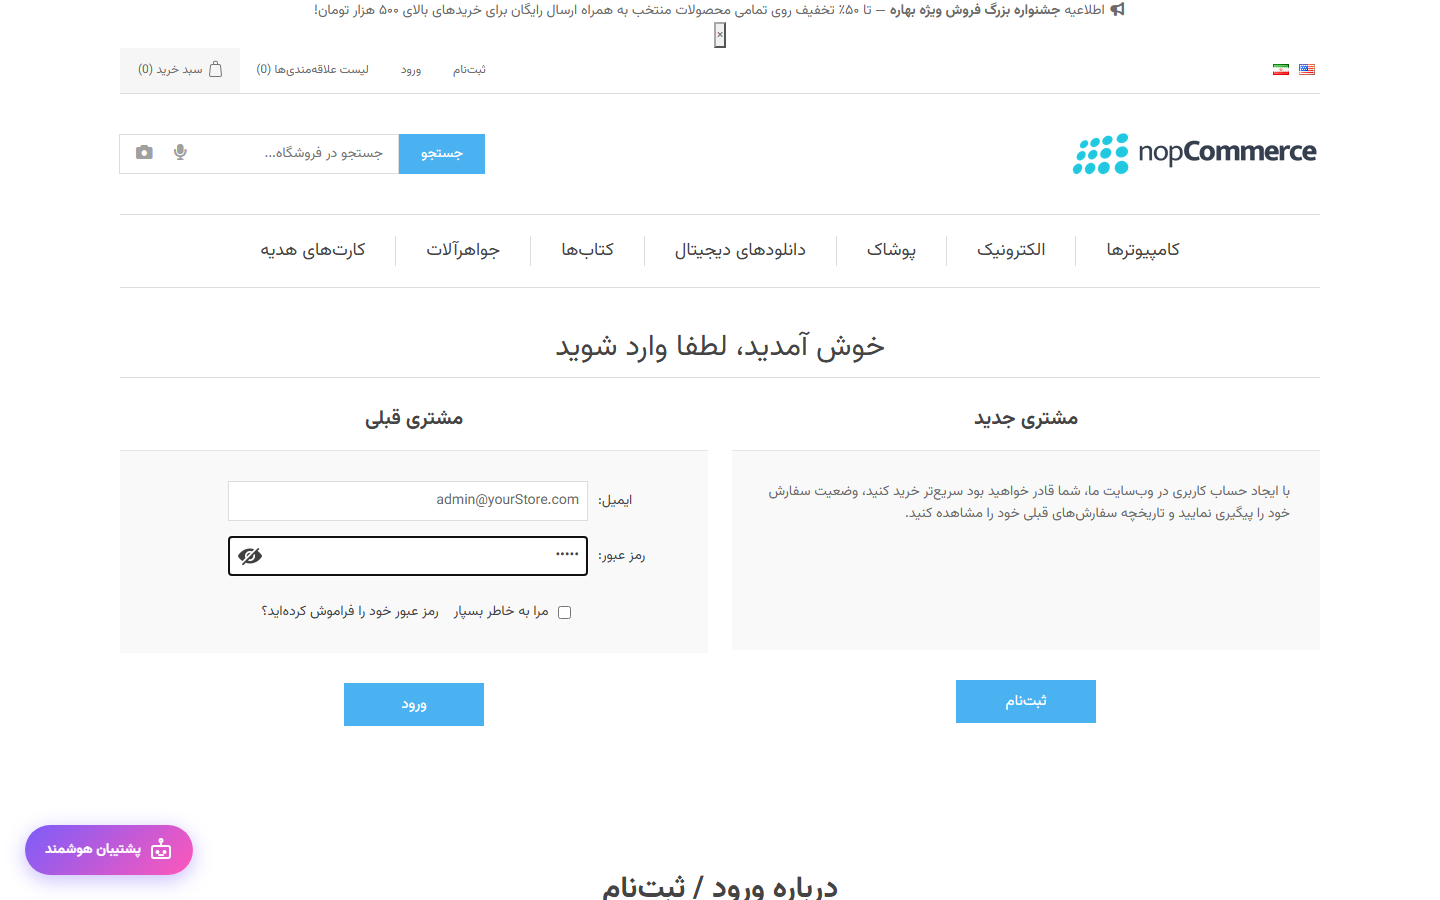
\includegraphics[width=0.88\textwidth]{images/mod1_01_persian_login.png}
\caption{گام ۱: صفحه ورود با تقویم شمسی و زبان فارسی}
\end{figure}

\begin{figure}[H]
\centering
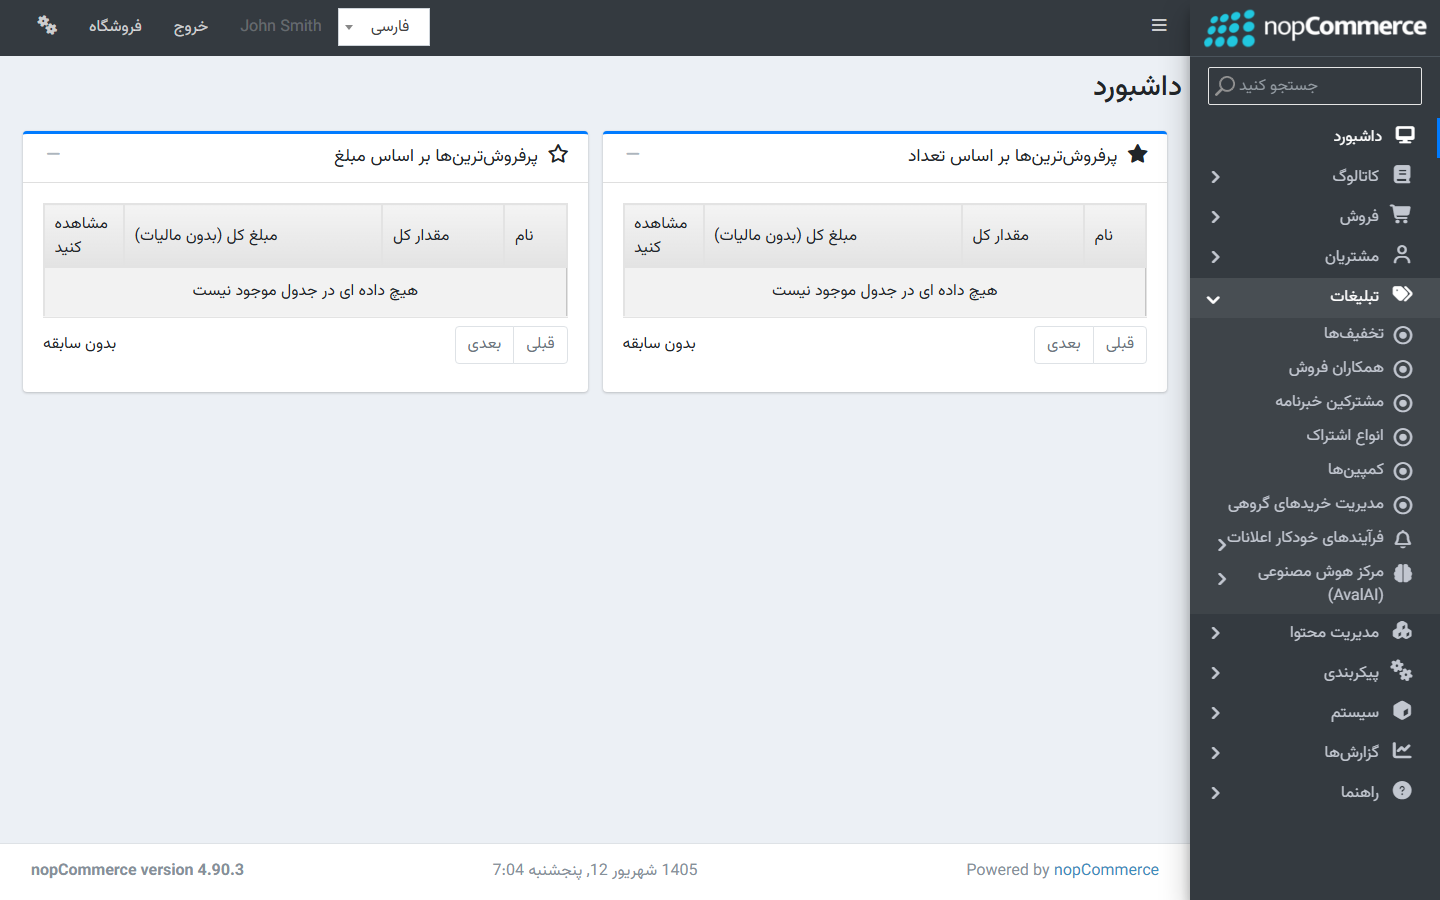
\includegraphics[width=0.88\textwidth]{images/mod1_02_admin_menu_persian.png}
\caption{گام ۲: منوی مدیریت اعلان‌ها در پنل ادمین فارسی}
\end{figure}

\begin{figure}[H]
\centering
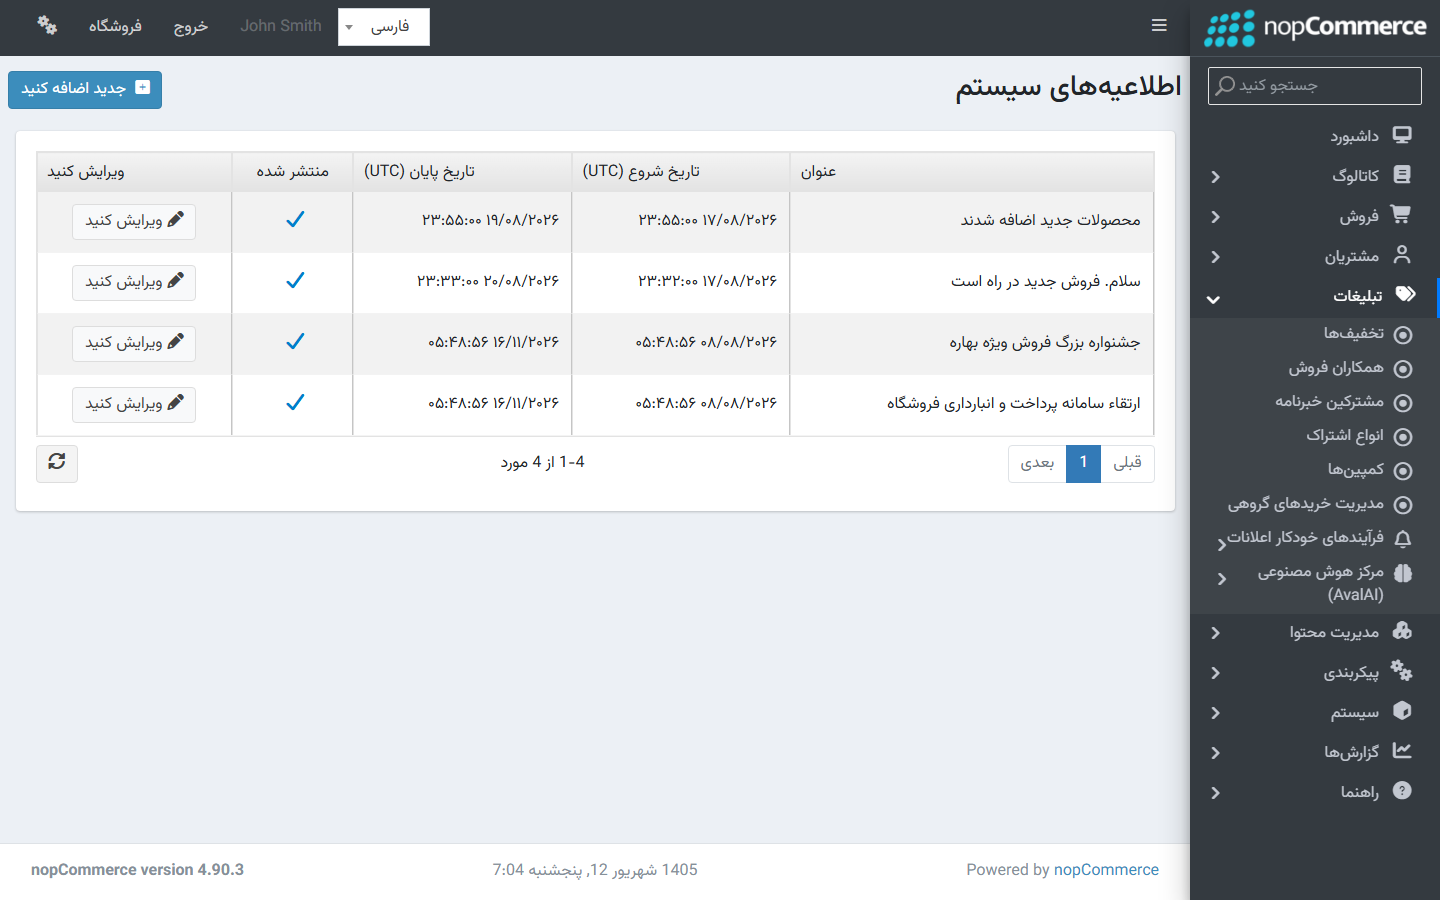
\includegraphics[width=0.88\textwidth]{images/mod1_03_announcements_list.png}
\caption{گام ۳: جدول لیست اطلاعیه‌ها و مدیریت وضعیت انتشار}
\end{figure}

\begin{figure}[H]
\centering
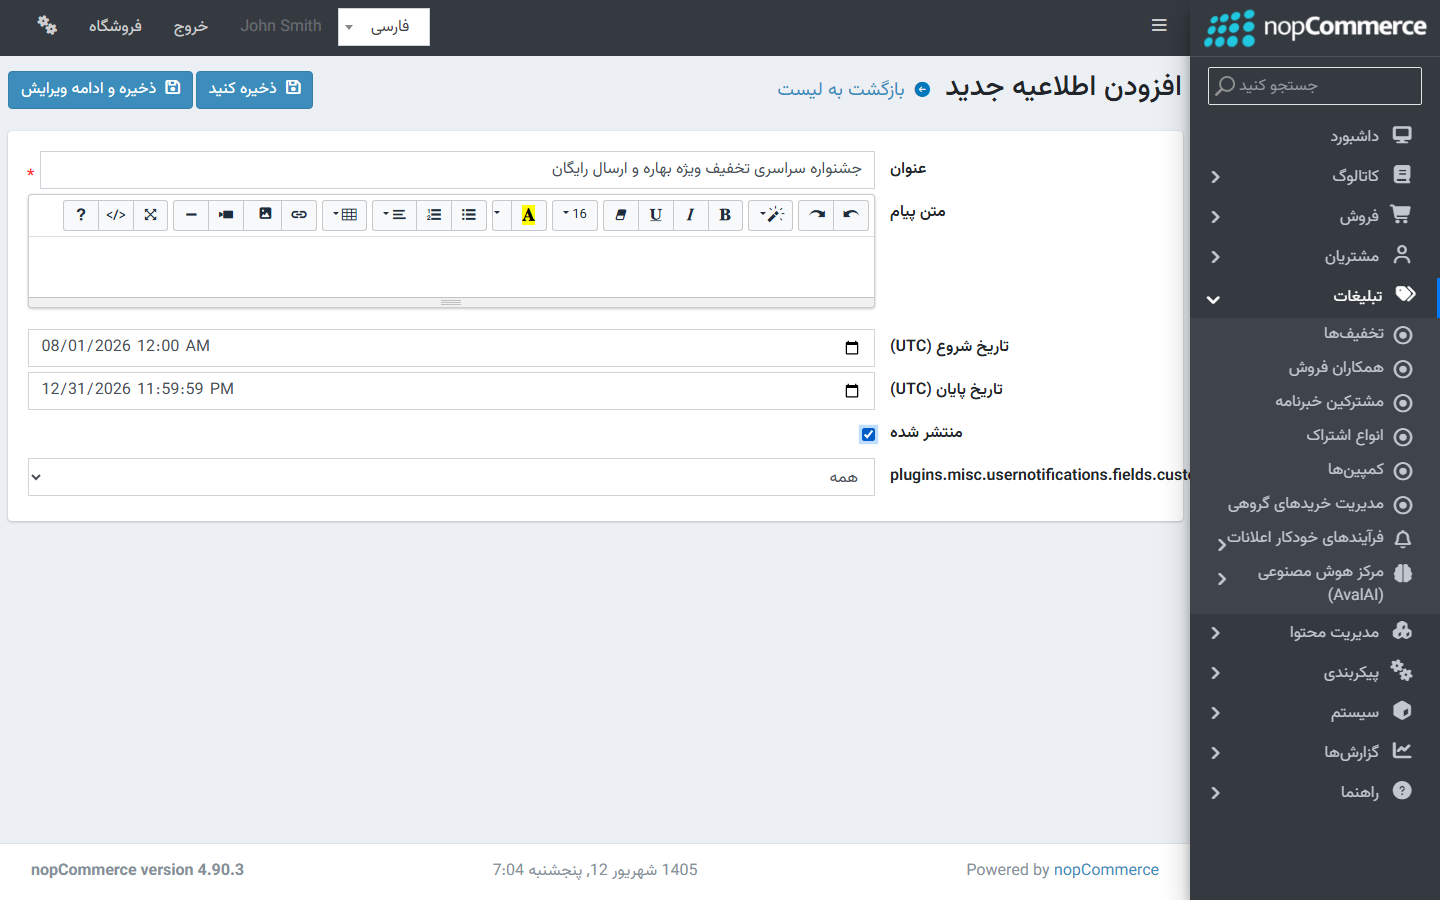
\includegraphics[width=0.88\textwidth]{images/mod1_04_create_announcement_form.png}
\caption{گام ۴: فرم تعریف اعلان جدید با تعیین نقش هدف و بازه زمانی}
\end{figure}

\begin{figure}[H]
\centering
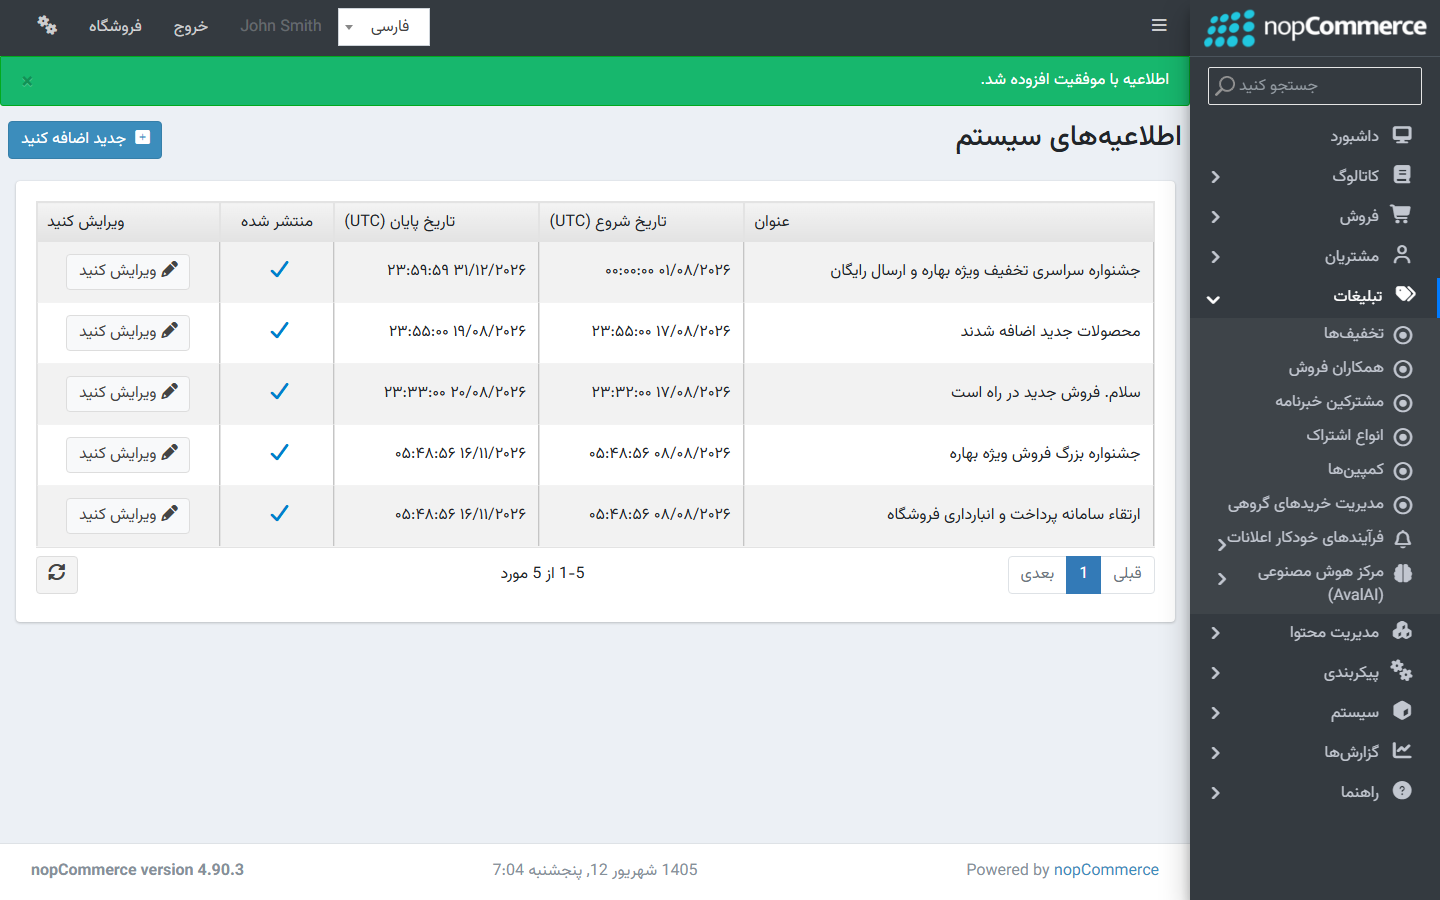
\includegraphics[width=0.88\textwidth]{images/mod1_05_announcement_created_success.png}
\caption{گام ۵: تایید موفقیت‌آمیز ثبت اعلان در دیتابیس فروشگاه}
\end{figure}

\begin{figure}[H]
\centering
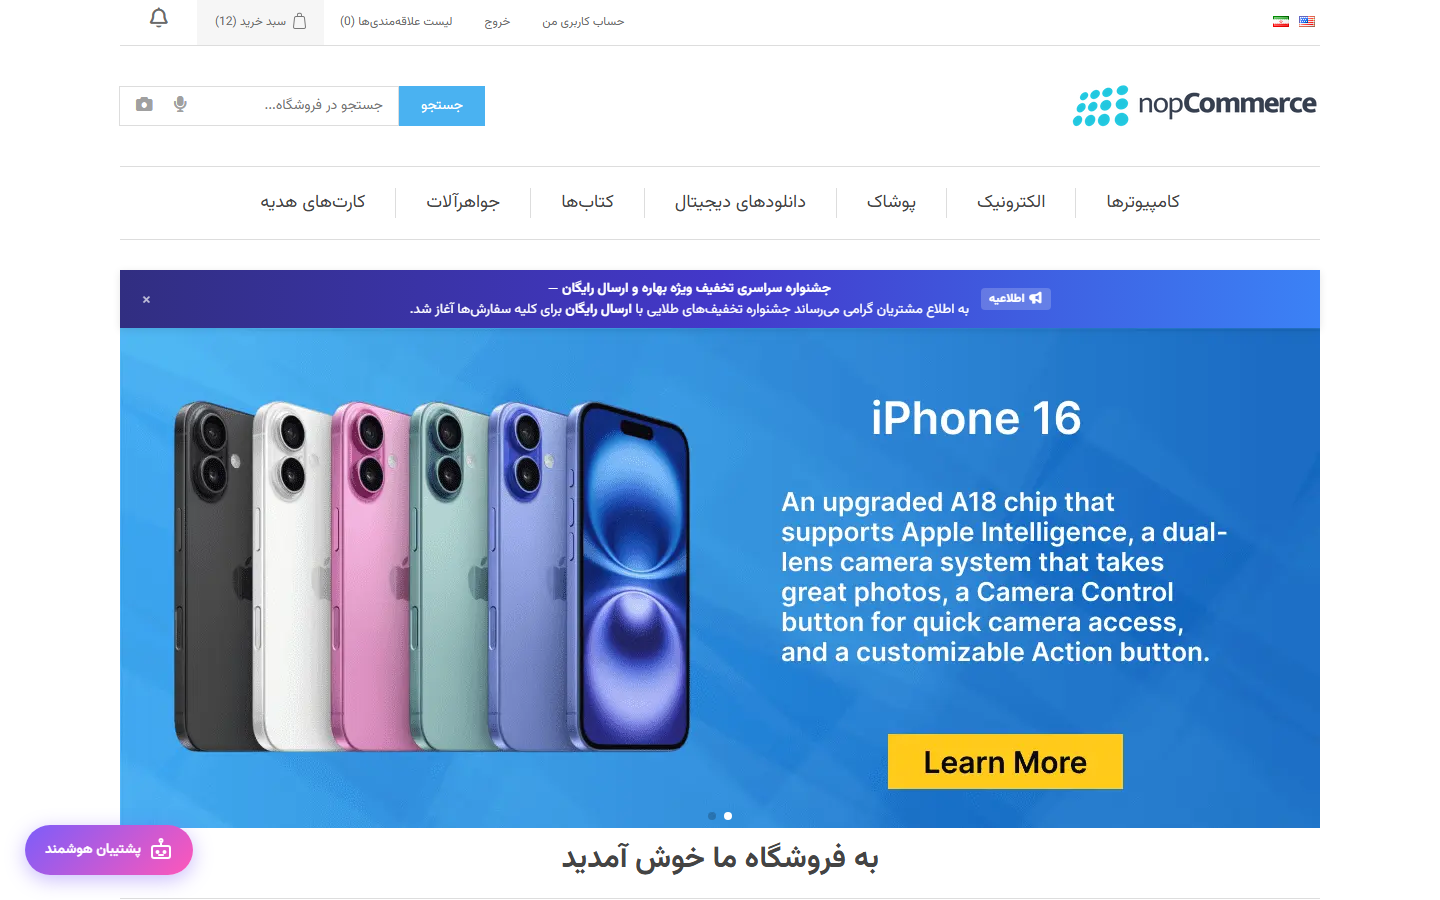
\includegraphics[width=0.88\textwidth]{images/mod1_06_storefront_persian_ticker.png}
\caption{گام ۶: بنر متحرک و نوتیفیکیشن زنده در بالای ویترین فروشگاه}
\end{figure}

\begin{figure}[H]
\centering
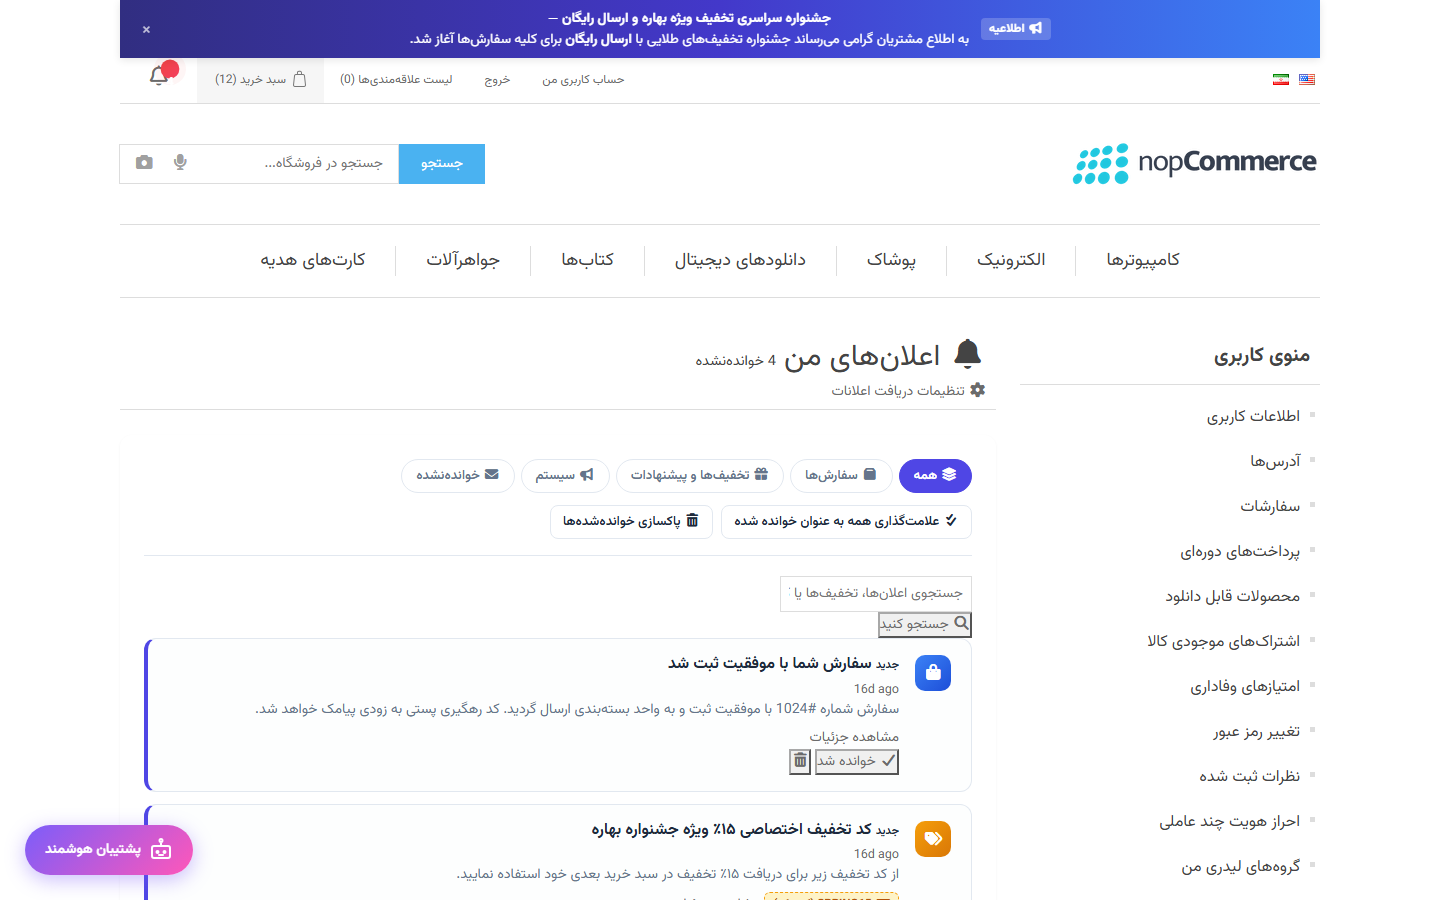
\includegraphics[width=0.88\textwidth]{images/mod1_07_customer_inbox.png}
\caption{گام ۷: صندوق پیام‌های شخصی در پنل حساب کاربری مشتری}
\end{figure}

\begin{figure}[H]
\centering
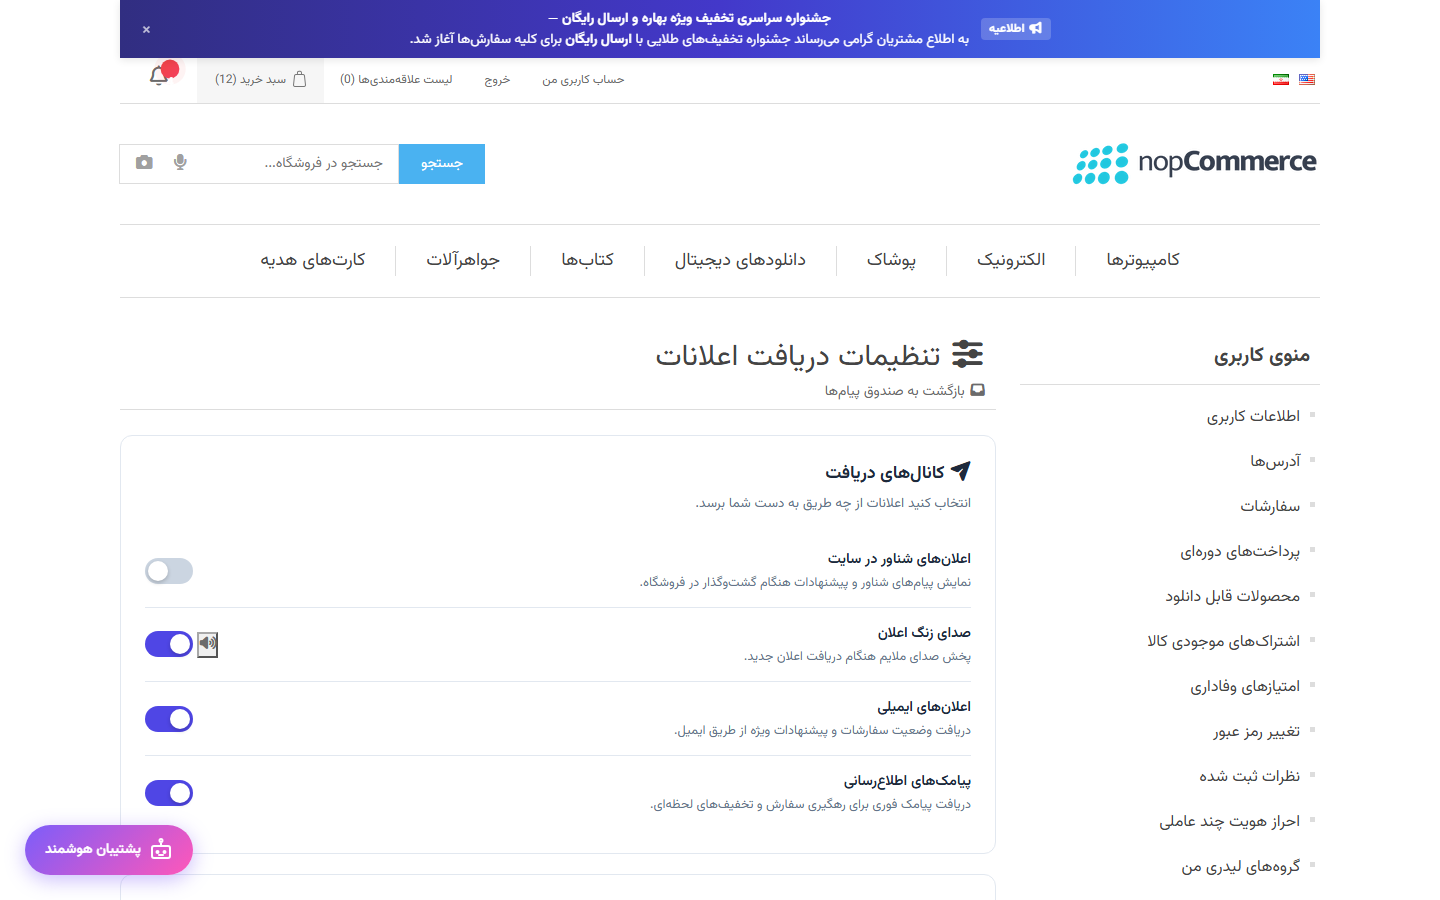
\includegraphics[width=0.88\textwidth]{images/mod1_08_customer_preferences.png}
\caption{گام ۸: تب تنظیمات ترجیحات دریافت پیام توسط مشتری}
\end{figure}

\begin{figure}[H]
\centering
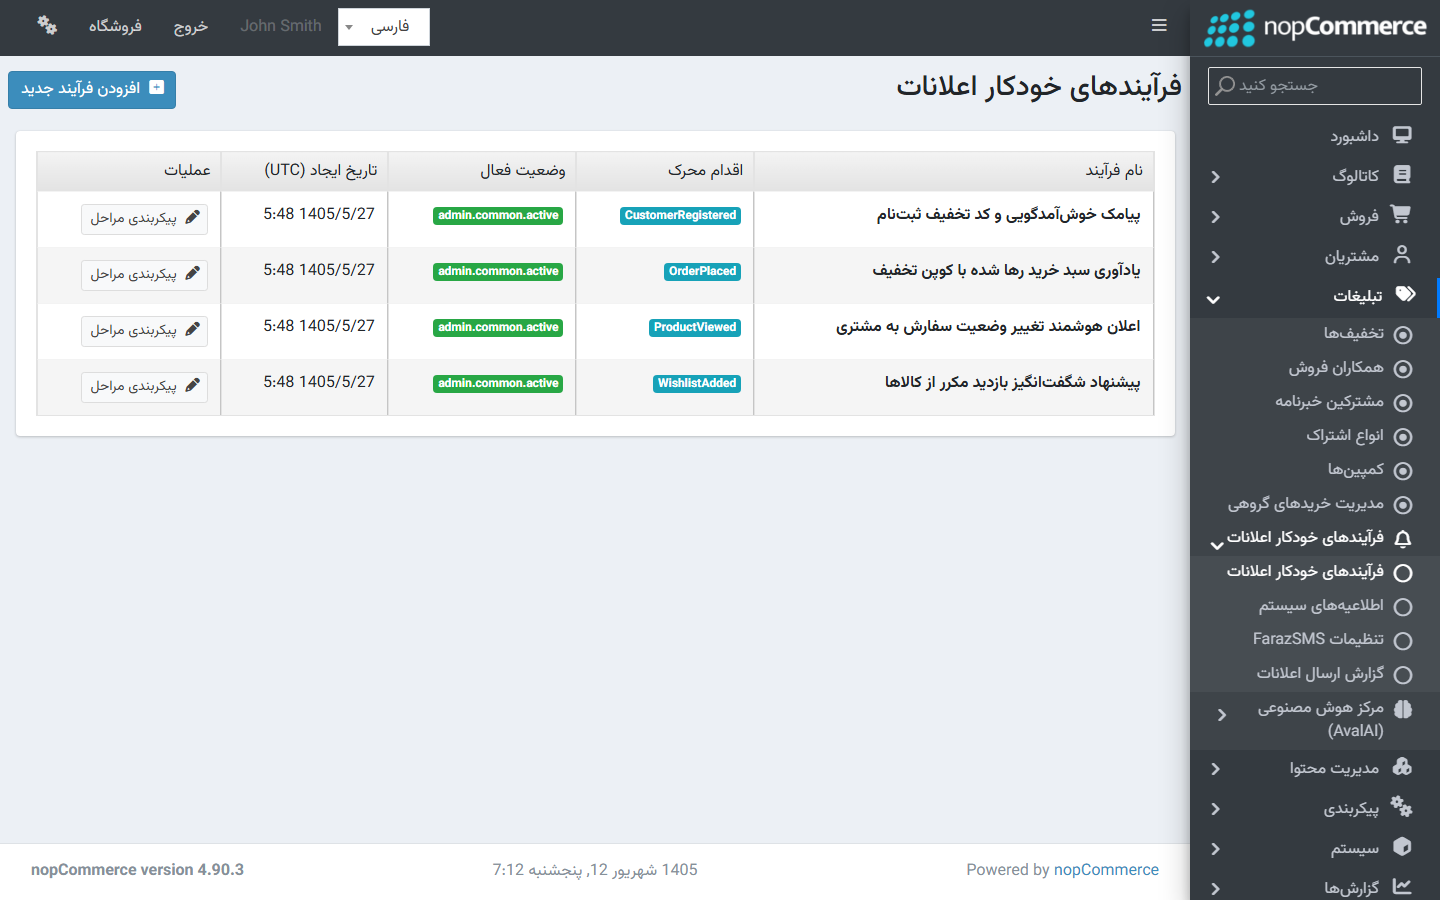
\includegraphics[width=0.88\textwidth]{images/mod1_09_automated_workflows.png}
\caption{گام ۹: جدول زمان‌بندی گردش‌کارهای خودکار سیستمی}
\end{figure}

\begin{figure}[H]
\centering
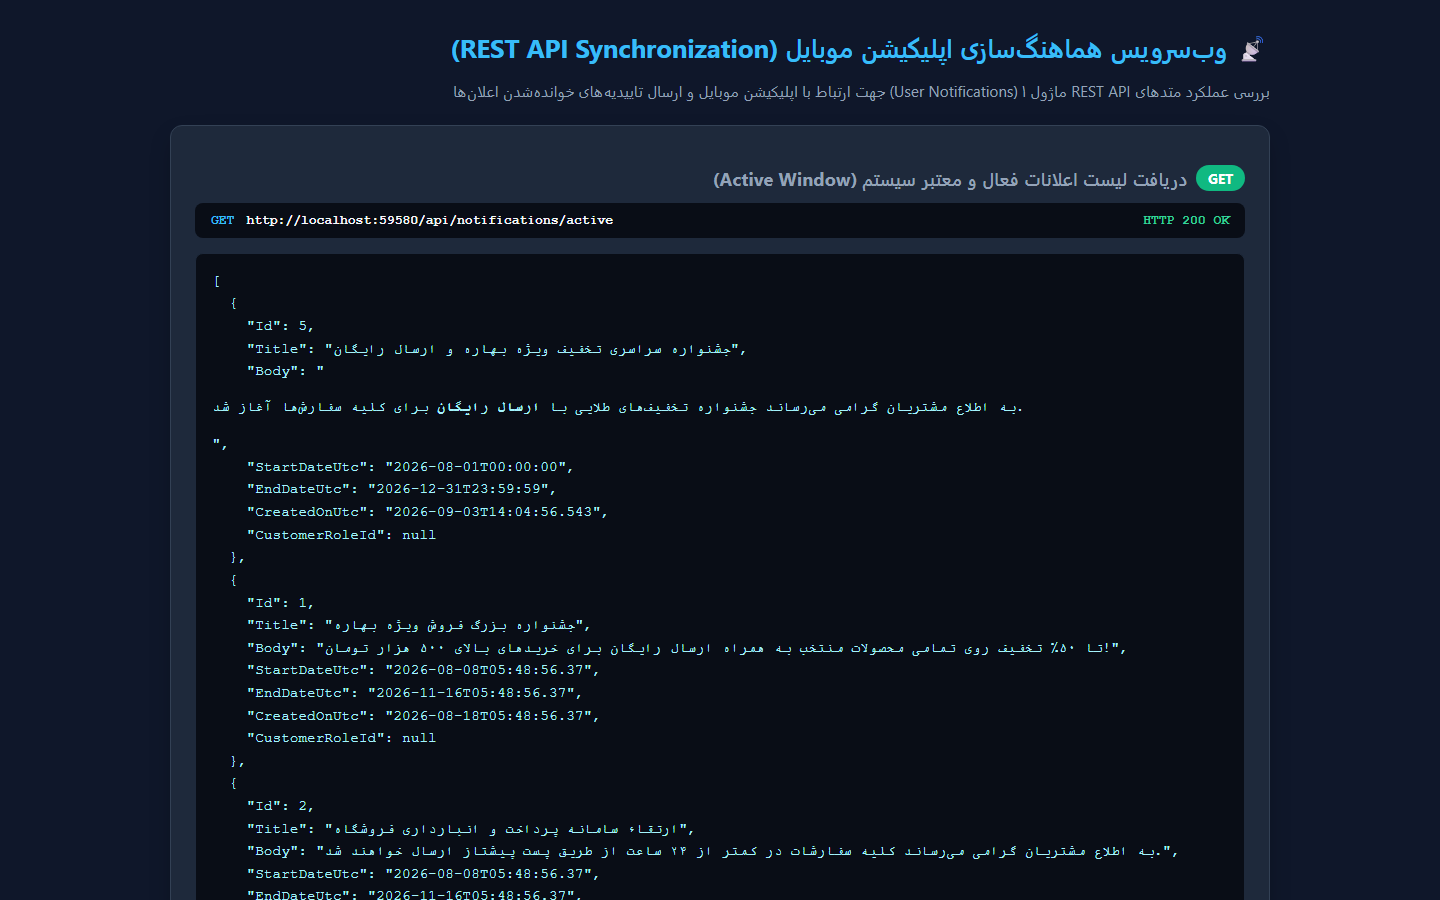
\includegraphics[width=0.88\textwidth]{images/mod1_10_mobile_rest_api.png}
\caption{گام ۱۰: اعتبارسنجی وب‌سرویس REST API با وضعیت HTTP 200 OK}
\end{figure}

\newpage

% -------------------------------------------------------------
% Chapter: Module 2
% -------------------------------------------------------------
\chapter[ماژول ۲: صفحه اختصاصی تخفیفات شگفت‌انگیز]{ماژول ۲: صفحه اختصاصی تخفیفات شگفت‌انگیز\\[0.3ex]\large\mdseries\lr{(Amazing Discounts)}}

\section{شرح کارکرد و ویژگی‌های ماژول}
این ماژول برای کمپین‌های فروش با تخفیف زمان‌دار (مشابه دیجی‌کالا) با ویژگی‌های زیر طراحی شده است:
\begin{enumerate}
    \item \textbf{صفحه لندینگ اختصاصی:} مسیر مستقیم \lr{/amazing-discounts} با طراحی بنر اختصاصی \lr{(Hero Banner)} و تم پرانرژی.
    \item \textbf{المان‌های ترغیب مشتری \lr{(FOMO)}:} تایمر معکوس زنده به تفکیک هر کالا، نوار پیشرفت موجودی فروخته‌شده \lr{(Stock Progress Bar)} و نشان‌های تخفیف درصدی.
    \item \textbf{نوار ناوبری ثابت پاورقی موبایل:} کامپوننت \lr{\#footer-navbar} جهت دسترسی دائمی کاربران تلفن همراه به بخش‌های خانه، تخفیفات، سبد خرید و پروفایل.
    \item \textbf{پیکربندی آسان ادمین:} قرارگیری منو در بخش استاندارد «تبلیغات» \lr{(Promotions)} جهت مدیریت آسان بازه‌ها و قیمت‌های شگفت‌انگیز.
\end{enumerate}

\section{مراحل ده‌گانه آزمون و مستندات تصویری ماژول ۲}

\begin{figure}[H]
\centering
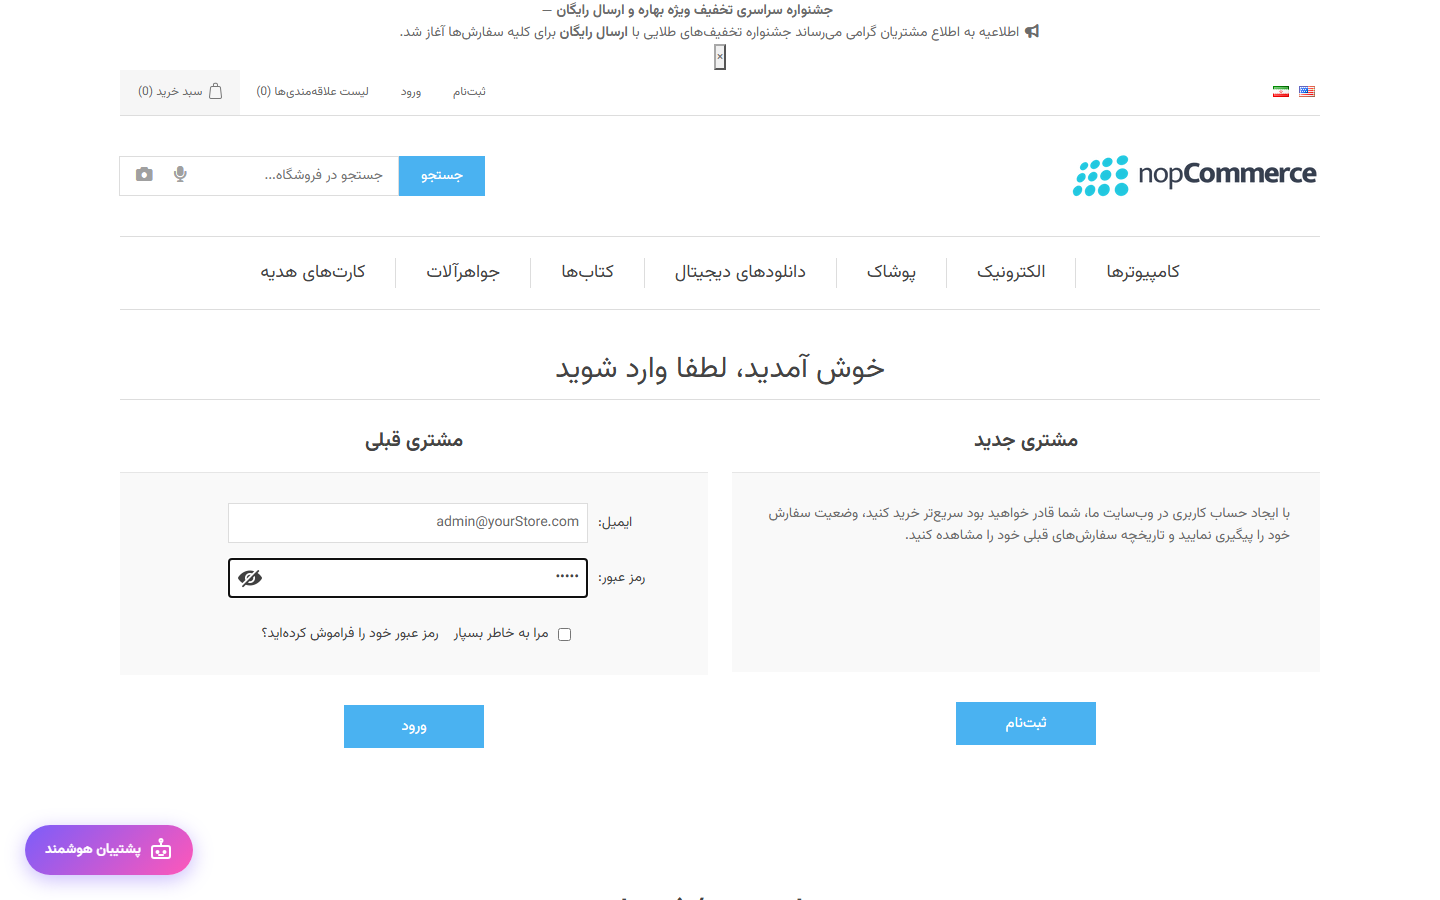
\includegraphics[width=0.88\textwidth]{images/mod2_01_persian_login.png}
\caption{گام ۱: احراز هویت ادمین با زبان فارسی}
\end{figure}

\begin{figure}[H]
\centering
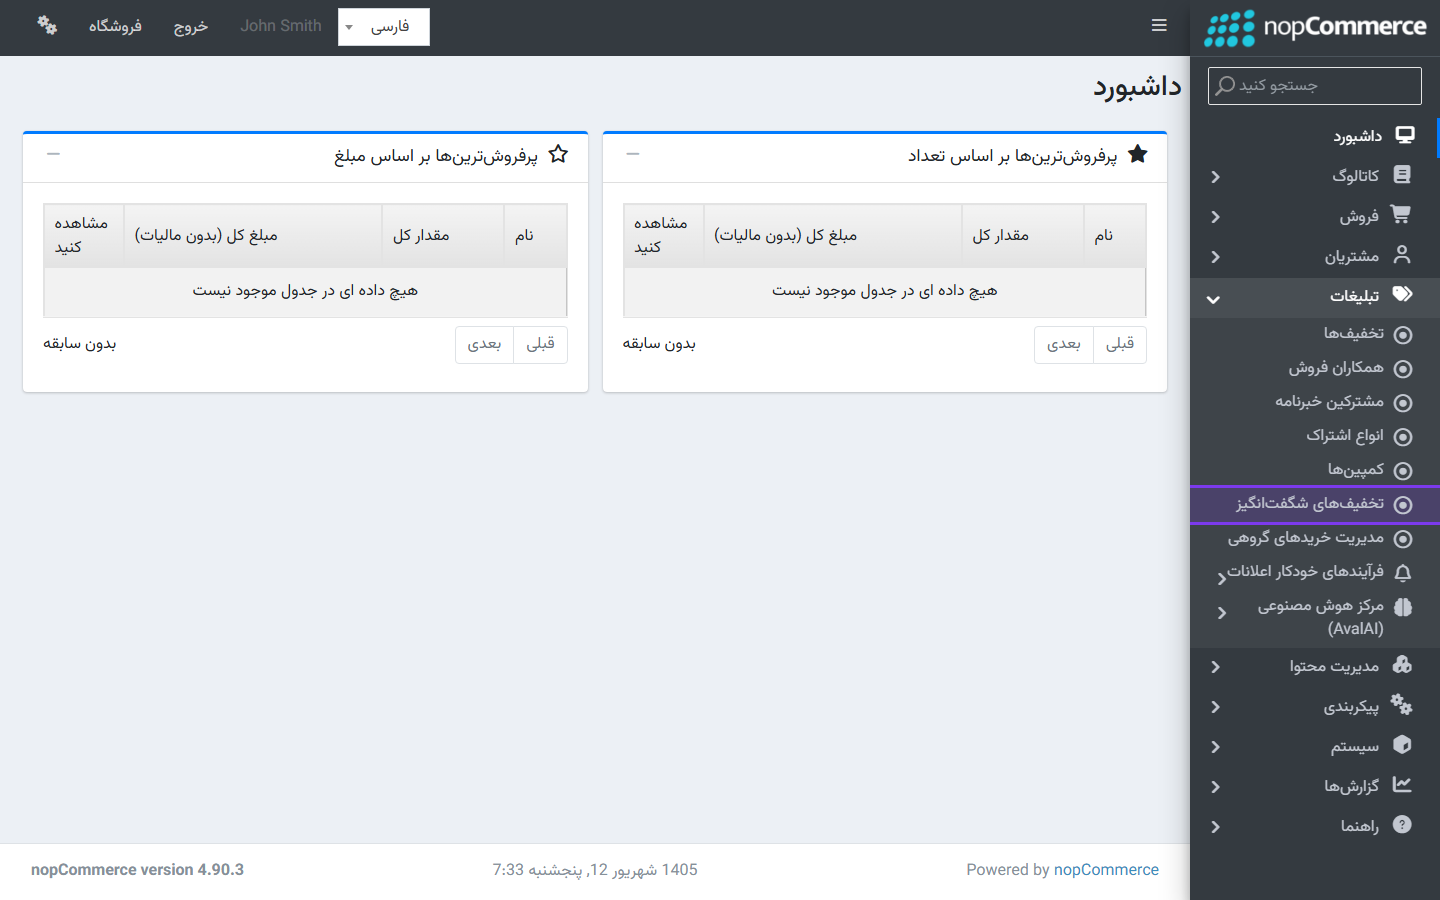
\includegraphics[width=0.88\textwidth]{images/mod2_02_admin_menu_promotions.png}
\caption{گام ۲: زیرمنوی تخفیفات شگفت‌انگیز در بخش تبلیغات}
\end{figure}

\begin{figure}[H]
\centering
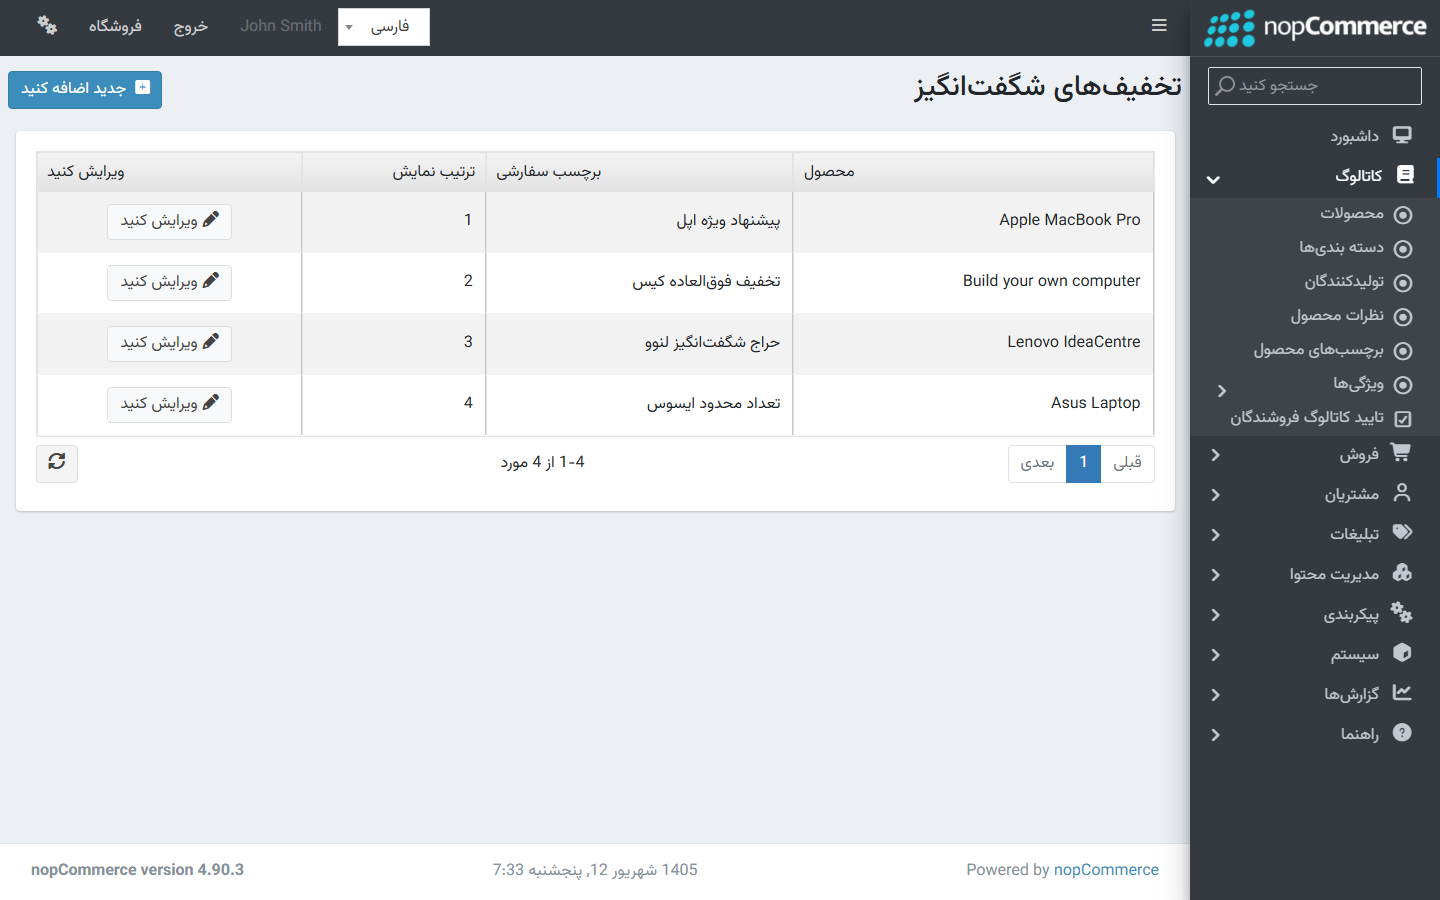
\includegraphics[width=0.88\textwidth]{images/mod2_03_amazing_discounts_grid.png}
\caption{گام ۳: جدول لیست پیشنهادهای شگفت‌انگیز با وضعیت فعال}
\end{figure}

\begin{figure}[H]
\centering
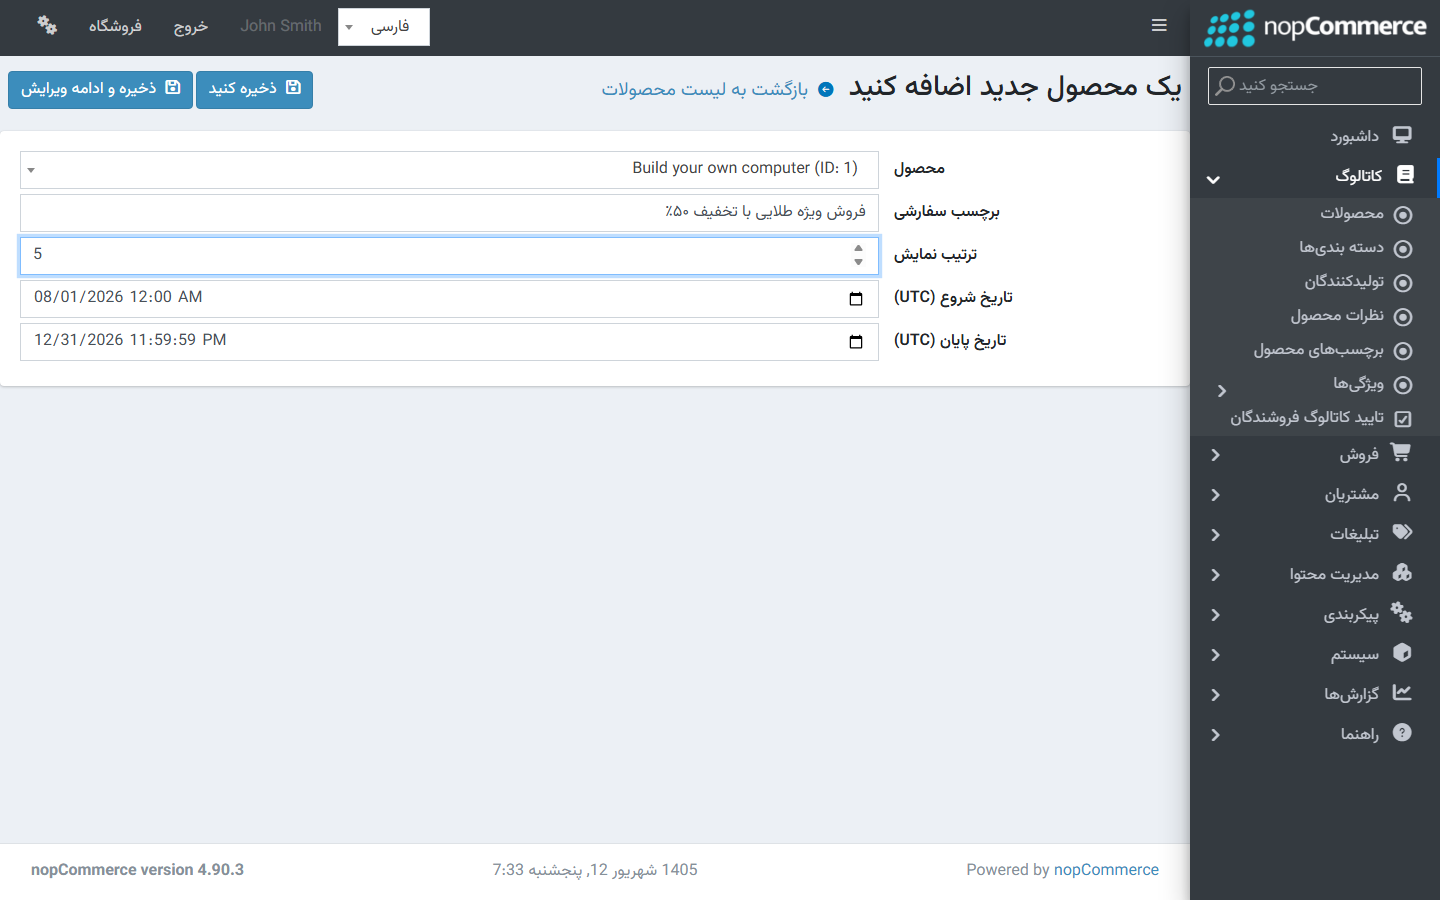
\includegraphics[width=0.88\textwidth]{images/mod2_04_create_amazing_discount.png}
\caption{گام ۴: فرم تعریف محصول شگفت‌انگیز و بازه زمانی انقضا}
\end{figure}

\begin{figure}[H]
\centering
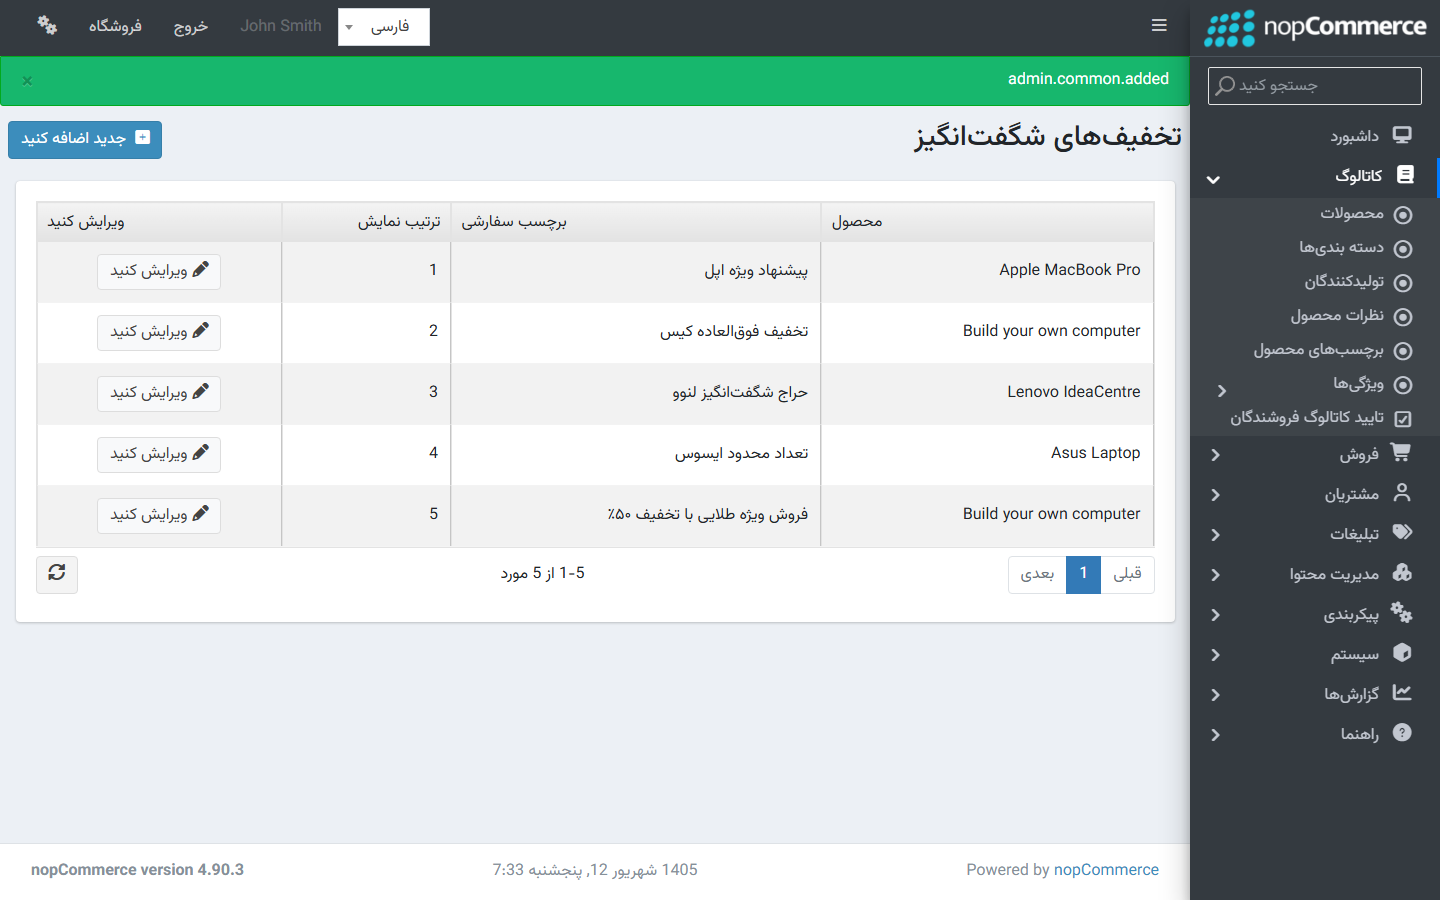
\includegraphics[width=0.88\textwidth]{images/mod2_05_discount_created_success.png}
\caption{گام ۵: تایید موفقیت‌آمیز درج پیشنهاد در سیستم}
\end{figure}

\begin{figure}[H]
\centering
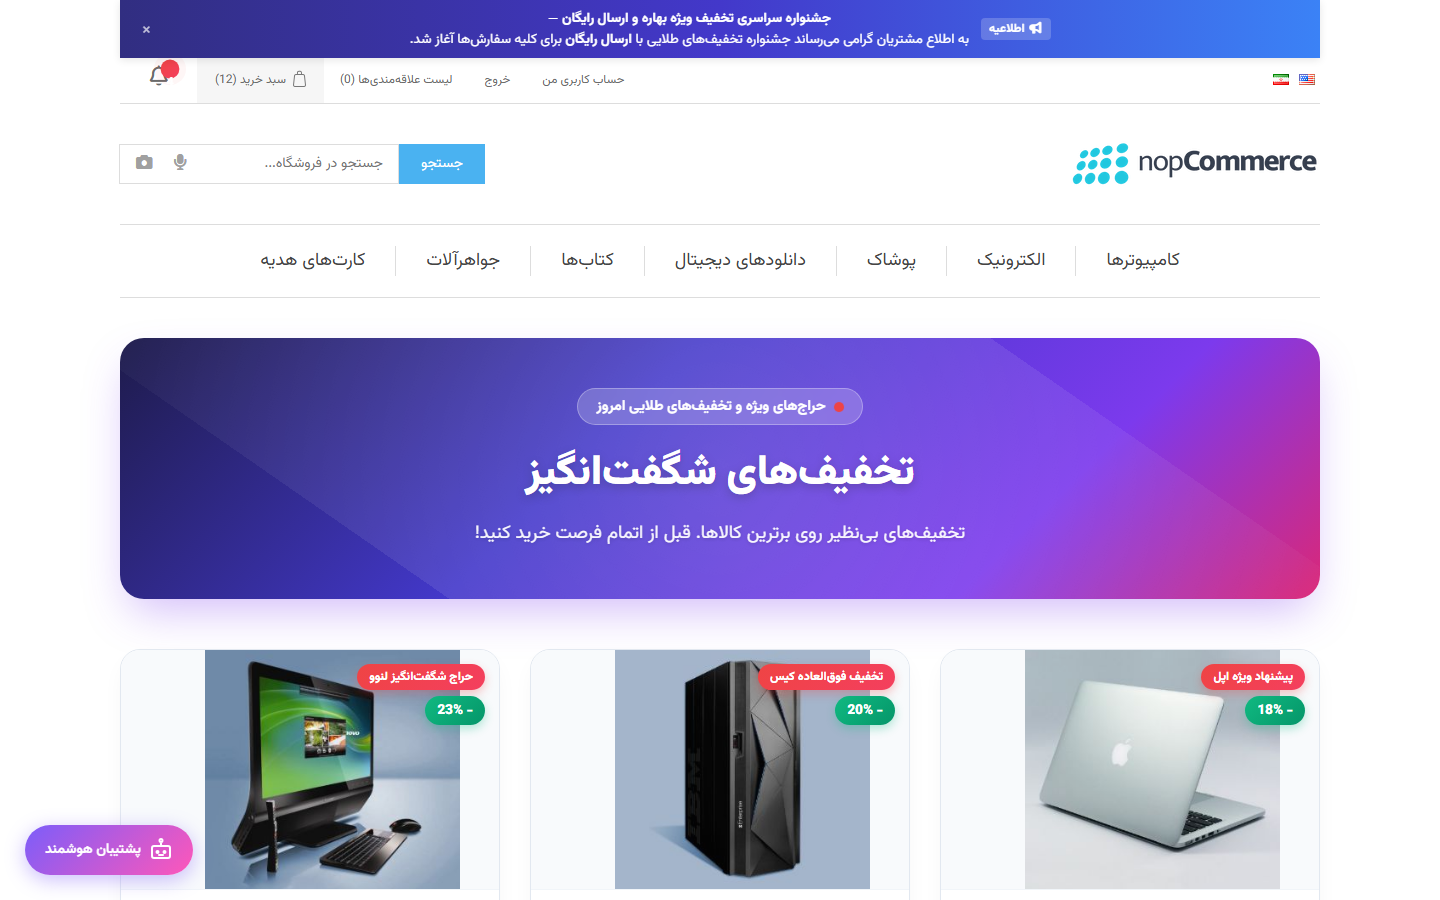
\includegraphics[width=0.88\textwidth]{images/mod2_06_storefront_landing_hero.png}
\caption{گام ۶: صفحه اصلی تخفیفات شگفت‌انگیز با بنر اختصاصی}
\end{figure}

\begin{figure}[H]
\centering
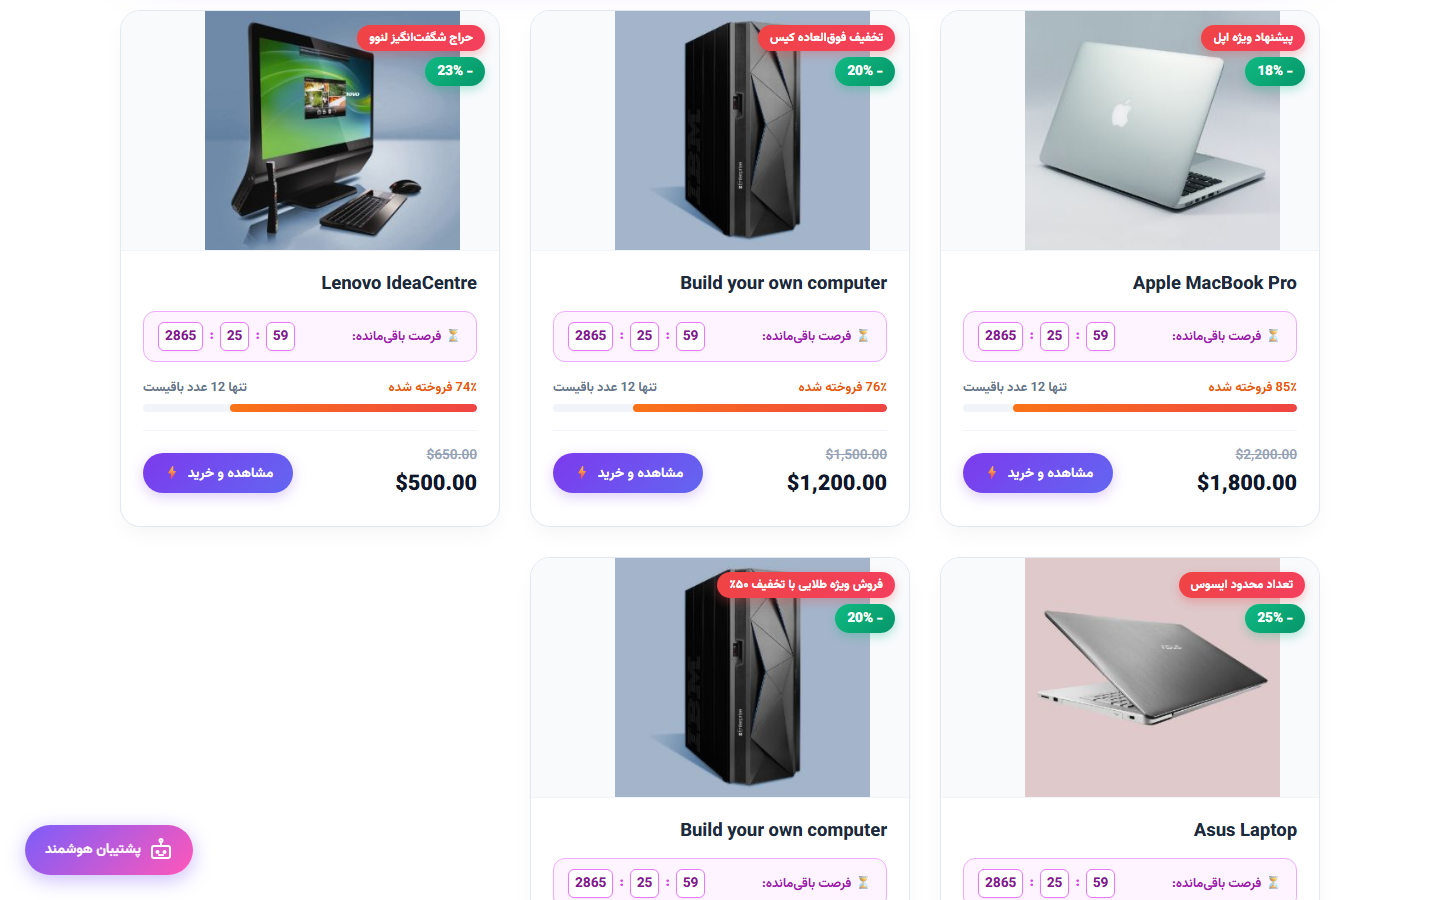
\includegraphics[width=0.88\textwidth]{images/mod2_07_deal_card_countdown_stock.png}
\caption{گام ۷: کارت‌های محصول همراه با ثانیه‌شمار معکوس و نوار موجودی}
\end{figure}

\begin{figure}[H]
\centering
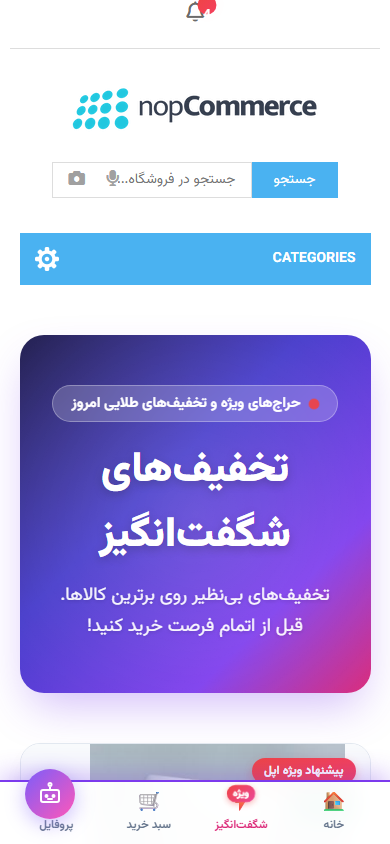
\includegraphics[width=0.88\textwidth]{images/mod2_08_mobile_footer_navbar.png}
\caption{گام ۸: نوار ناوبری ثابت در پایین صفحه نمایش موبایل}
\end{figure}

\begin{figure}[H]
\centering
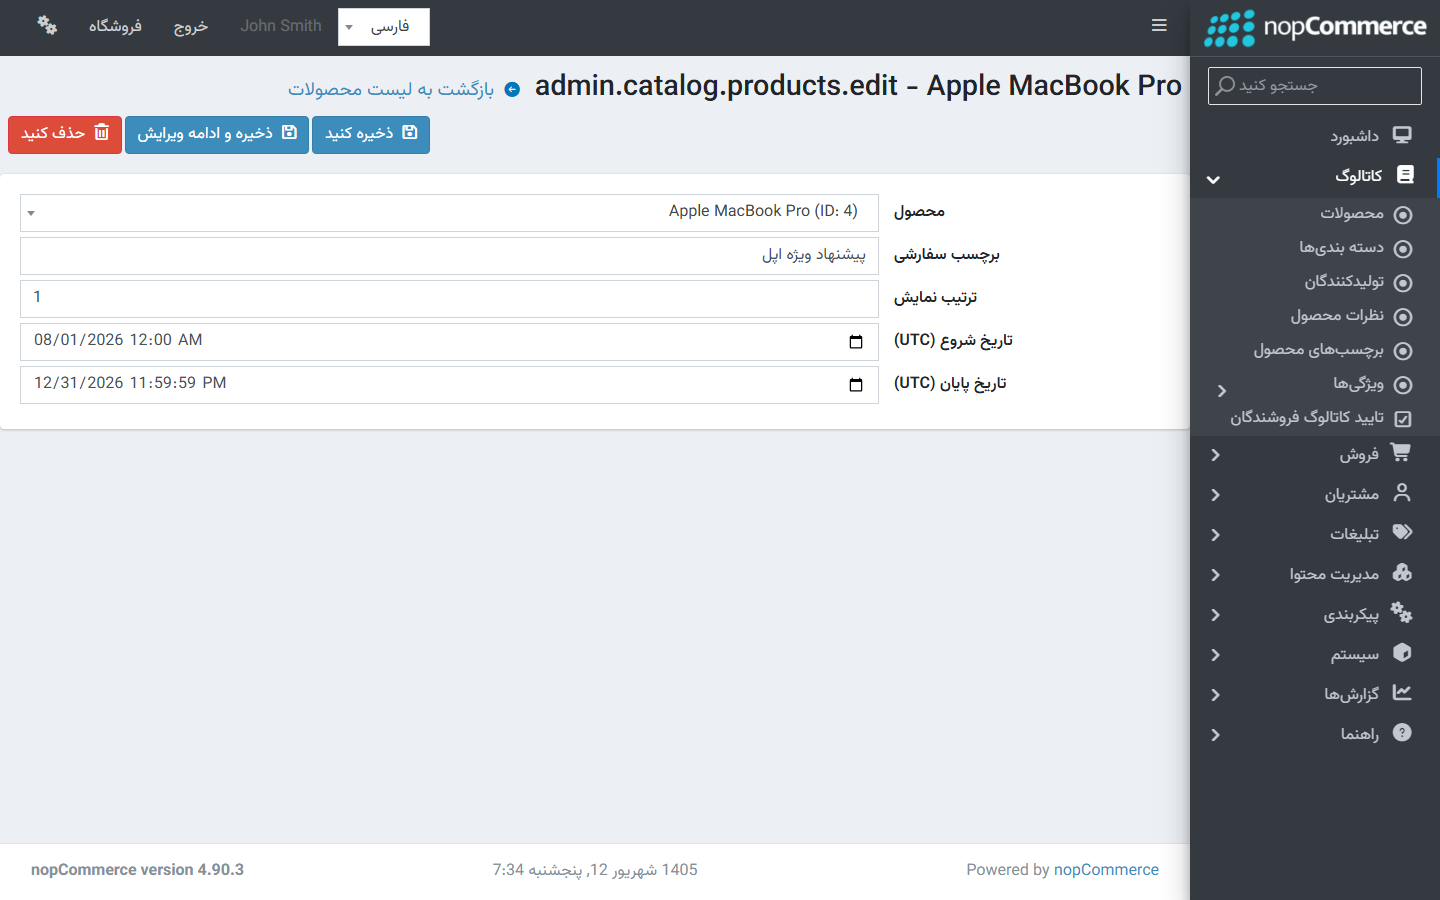
\includegraphics[width=0.88\textwidth]{images/mod2_09_edit_amazing_discount.png}
\caption{گام ۹: فرم ویرایش و تمدید بازه تخفیف شگفت‌انگیز}
\end{figure}

\begin{figure}[H]
\centering
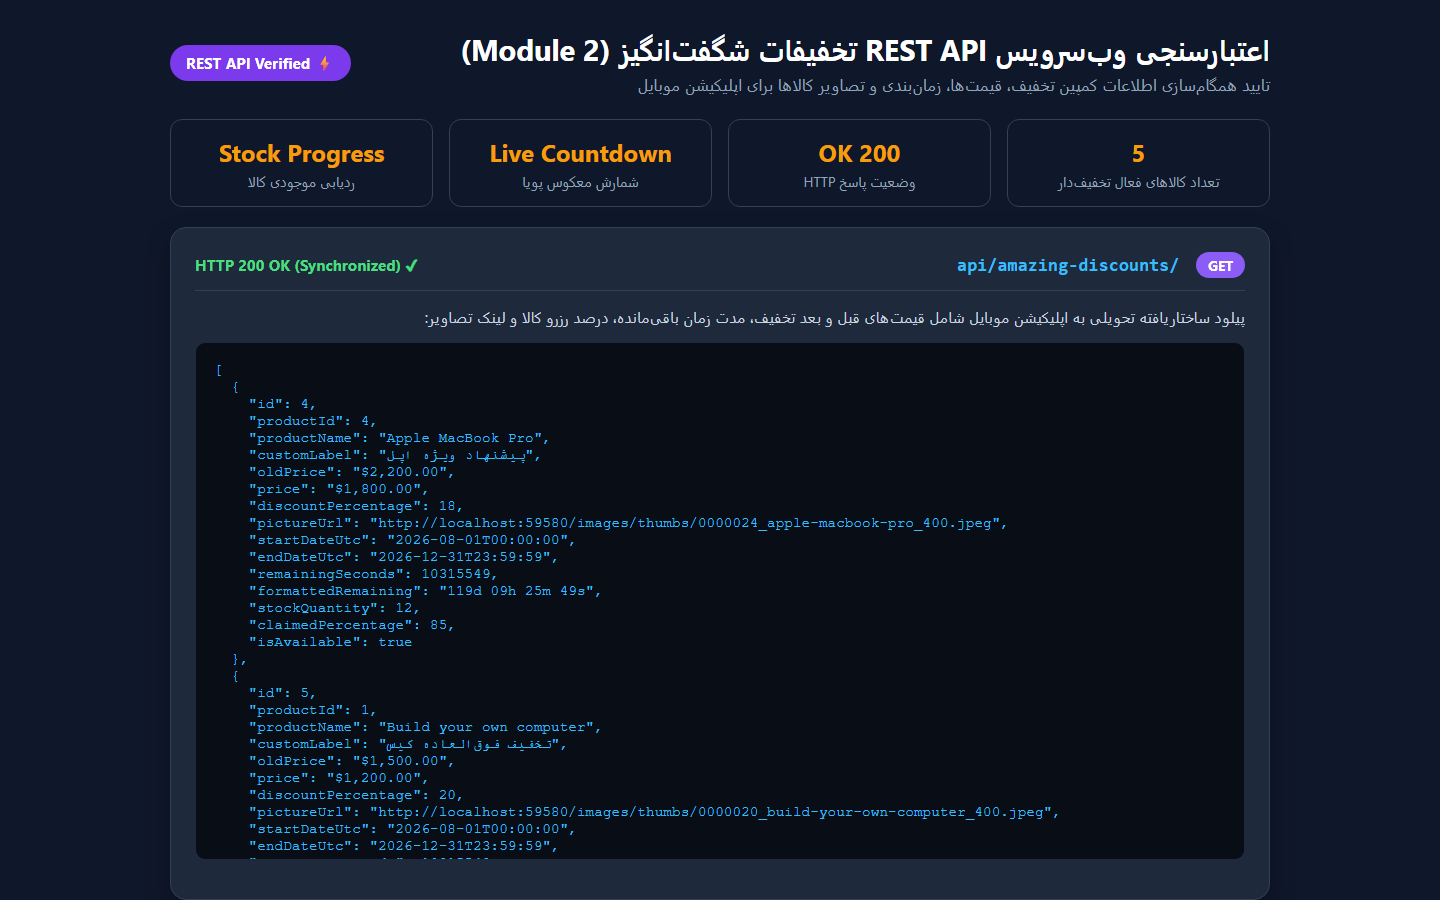
\includegraphics[width=0.88\textwidth]{images/mod2_10_mobile_rest_api.png}
\caption{گام ۱۰: خروجی وب‌سرویس REST API تخفیفات شگفت‌انگیز برای موبایل}
\end{figure}

\newpage

% -------------------------------------------------------------
% Chapter: Module 3
% -------------------------------------------------------------
\chapter[ماژول ۳: سامانه پیشرفته خرید گروهی و اشتراکی]{ماژول ۳: سامانه پیشرفته خرید گروهی و اشتراکی\\[0.3ex]\large\mdseries\lr{(Group Buying)}}

\section{شرح کارکرد و نیازمندی‌های سیستم}
این ماژول پیشرفته با ایجاد انگیزه اجتماعی و پاداش‌های چندسطحی، نرخ تبدیل و حجم سفارشات را افزایش می‌دهد:
\begin{enumerate}
    \item \textbf{ورودی سبد خرید و کد اختصاصی:} تبدیل آسان سبد به خرید گروهی و صدور کد یکتای اشتراک \lr{(مانند \texttt{GP-78241})}.
    \item \textbf{تعهدنامه حقوقی و لاگ رسمی:} ثبت تاییدیه صریح «می‌پذیرم» سرگروه (مسئولیت امانی تحویل کالا) و عضو همراه با آدرس \lr{IP} و متن پیام در \lr{GP\_LegalConfirmationLog}.
    \item \textbf{حفظ حریم خصوصی اعضا:} انتخاب سطح محرمانگی در ۳ حالت: نمایش کامل، نمایش محدود فقط تعداد، یا عدم نمایش اقلام سبد به سرگروه.
    \item \textbf{موتور پاداش چندسطحی ادمین:} پشتیبانی از ۷ نوع پاداش (شارژ کیف پول، تخفیف سبد، اشانتیون، پیک رایگان و...) بر پایه درصد از سبد یا سود خالص.
    \item \textbf{مکانیزم قفل‌گذاری و باشگاه مشتریان:} پاداش‌های اعضای زیرگروه تا ۵ سفارش موفق قفل می‌ماند؛ امتیازات با فرمول دوگانه (۱ امتیاز = ۲۰,۰۰۰ تومان اعتبار یا ۱ شانس قرعه‌کشی) مدیریت می‌شود.
\end{enumerate}

\section{مراحل یازده‌گانه آزمون و مستندات تصویری ماژول ۳}

\begin{figure}[H]
\centering
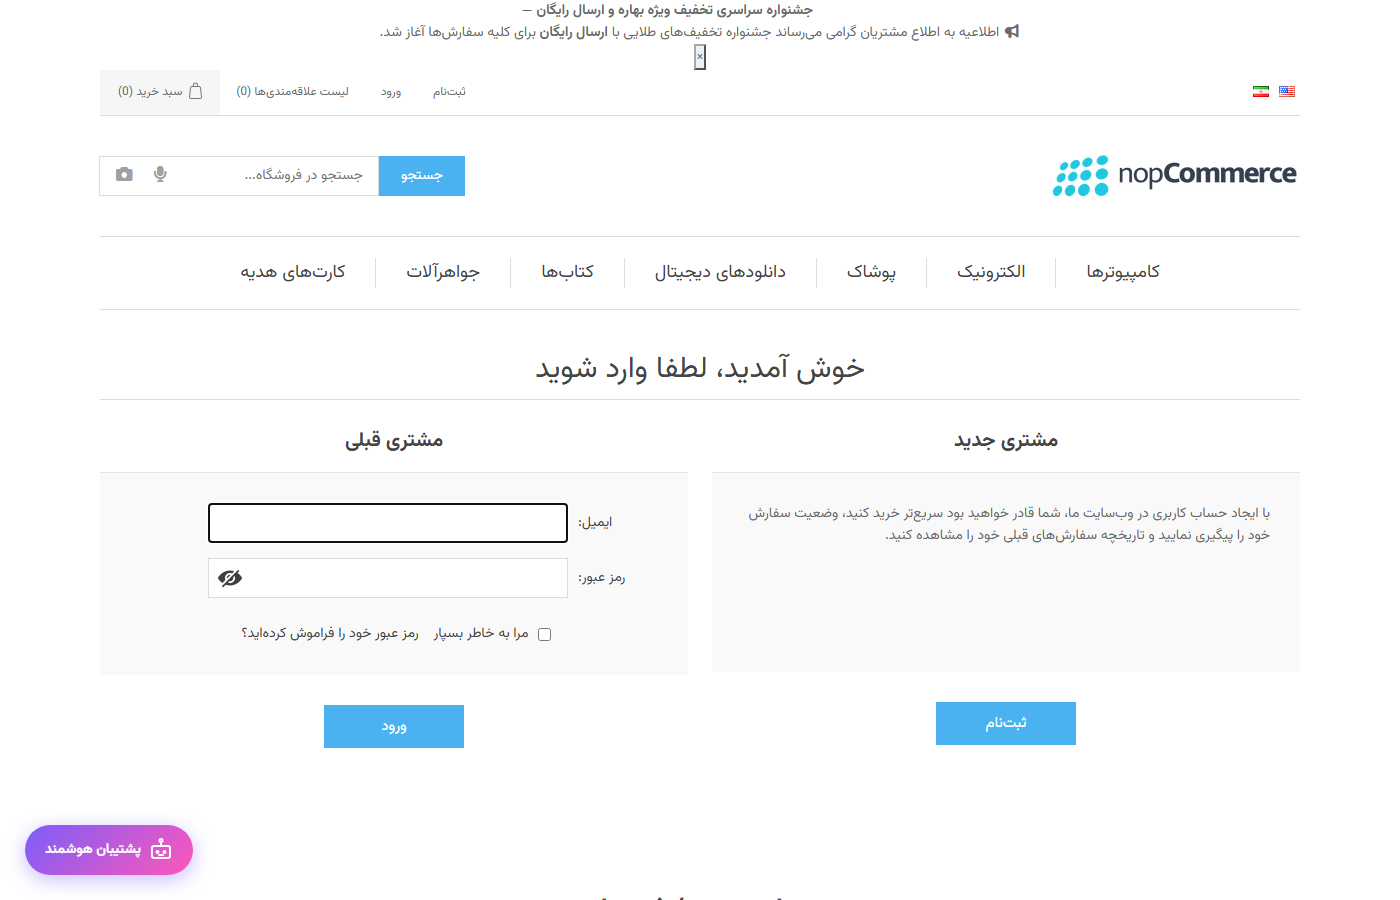
\includegraphics[width=0.88\textwidth]{images/mod3_01_persian_login.png}
\caption{گام ۱: ورود به فروشگاه با زبان فارسی}
\end{figure}

\begin{figure}[H]
\centering
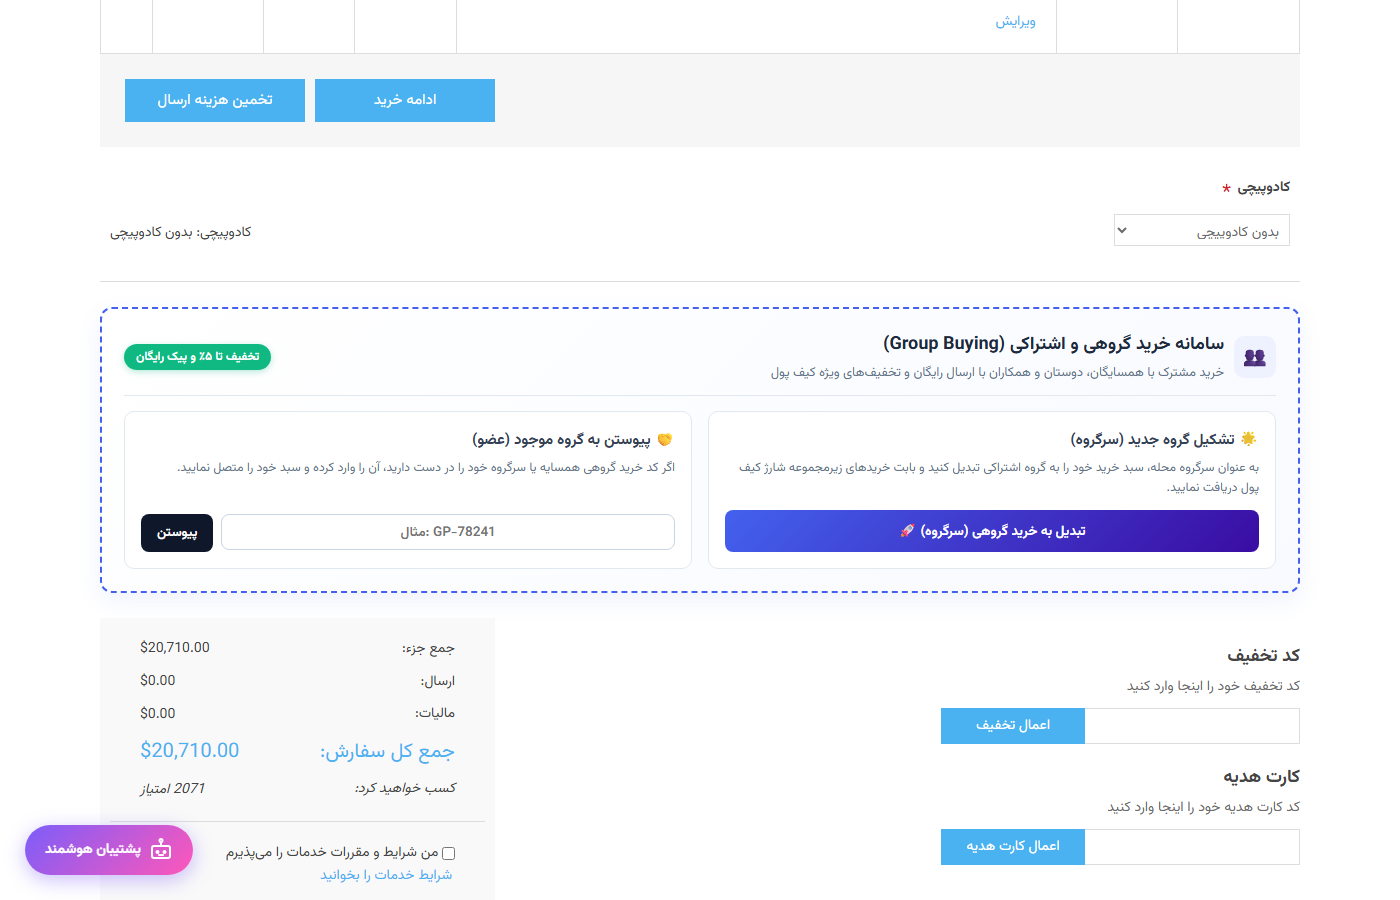
\includegraphics[width=0.88\textwidth]{images/mod3_02_cart_group_purchase_widget.png}
\caption{گام ۲: ویجت خرید گروهی در سبد خرید با گزینه‌های سرگروه و عضو}
\end{figure}

\begin{figure}[H]
\centering
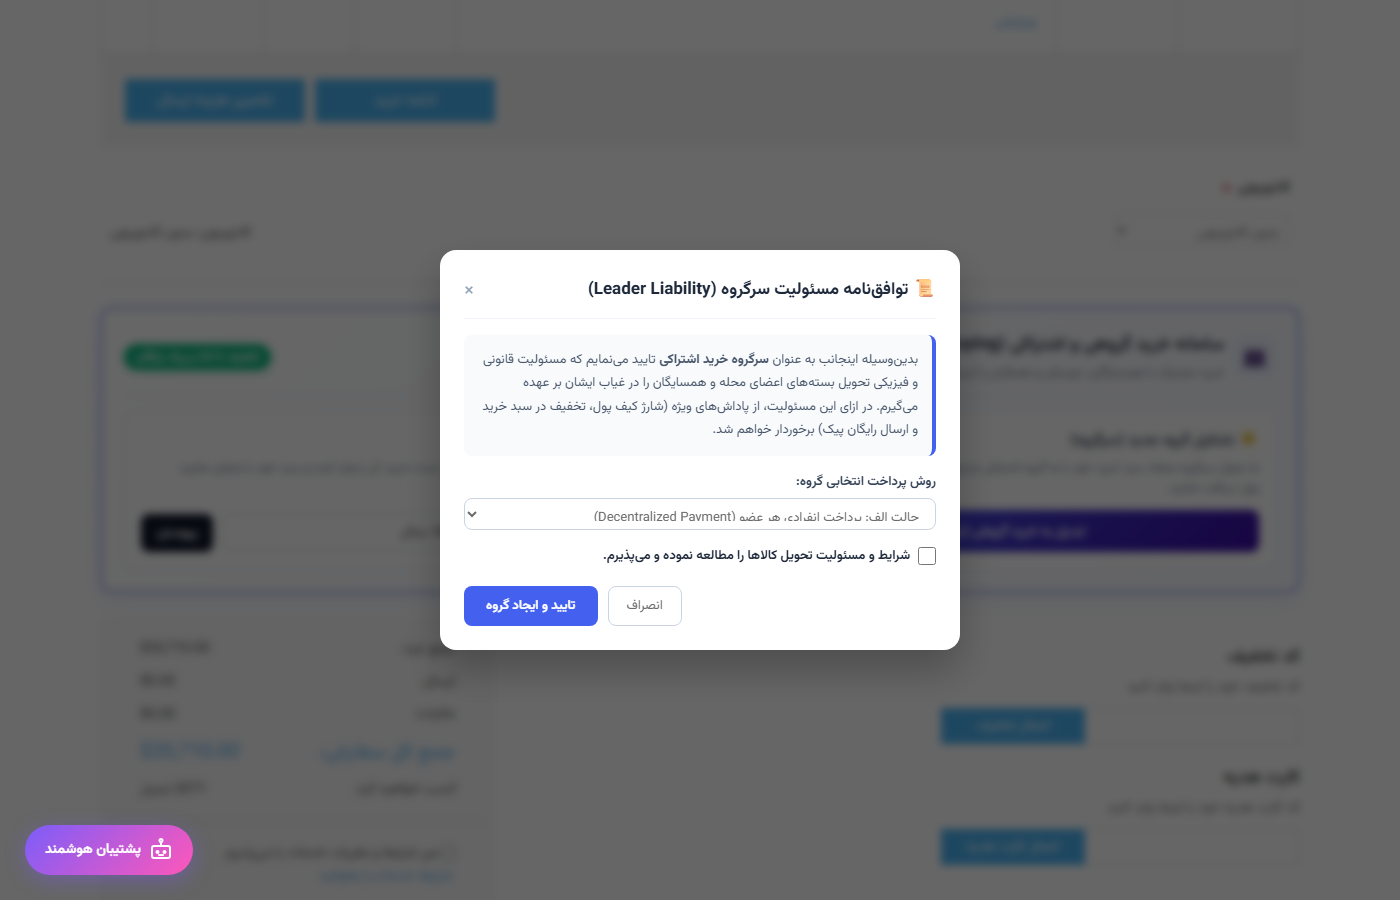
\includegraphics[width=0.88\textwidth]{images/mod3_03_leader_liability_modal.png}
\caption{گام ۳: مودال توافق‌نامه مسئولیت حقوقی سرگروه و انتخاب شیوه پرداخت}
\end{figure}

\begin{figure}[H]
\centering
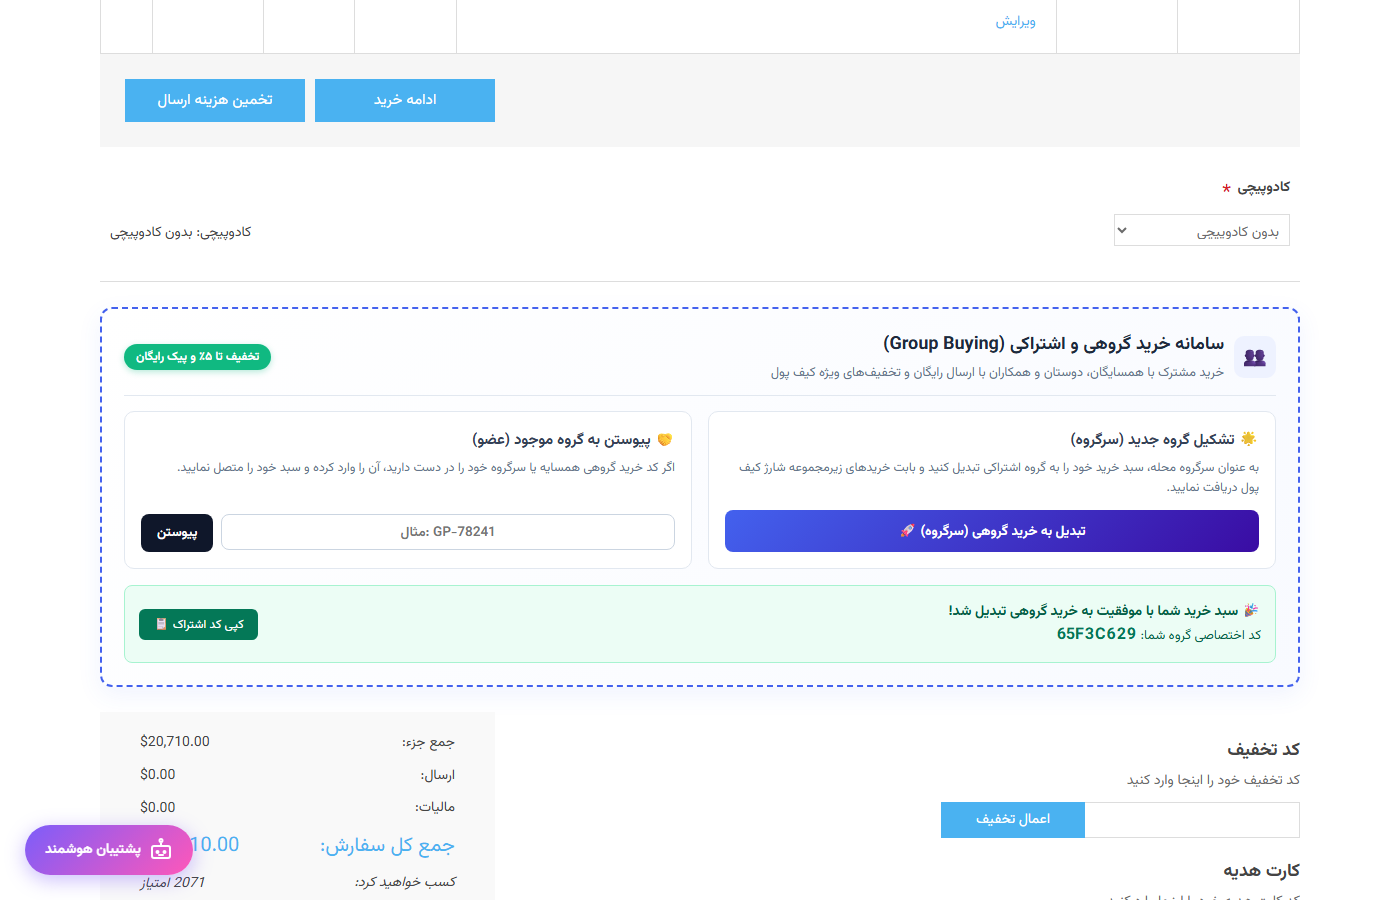
\includegraphics[width=0.88\textwidth]{images/mod3_04_group_code_created.png}
\caption{گام ۴: صدور کد اختصاصی خرید گروهی با دکمه کپی در کلیپ‌بورد}
\end{figure}

\begin{figure}[H]
\centering
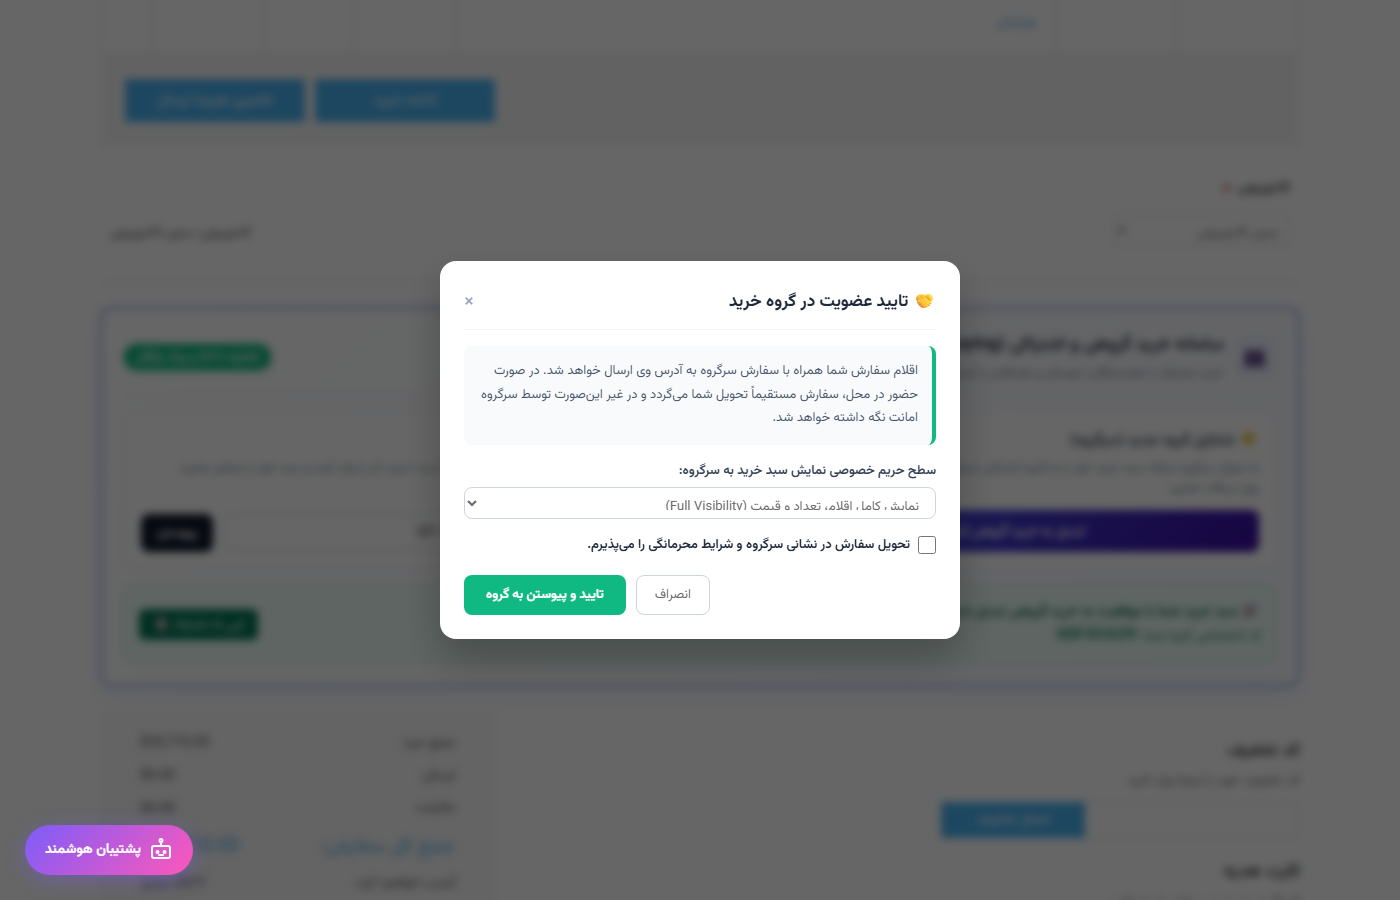
\includegraphics[width=0.88\textwidth]{images/mod3_05_member_join_modal.png}
\caption{گام ۵: مودال تایید عضویت عضو و انتخاب سطح حریم خصوصی}
\end{figure}

\begin{figure}[H]
\centering
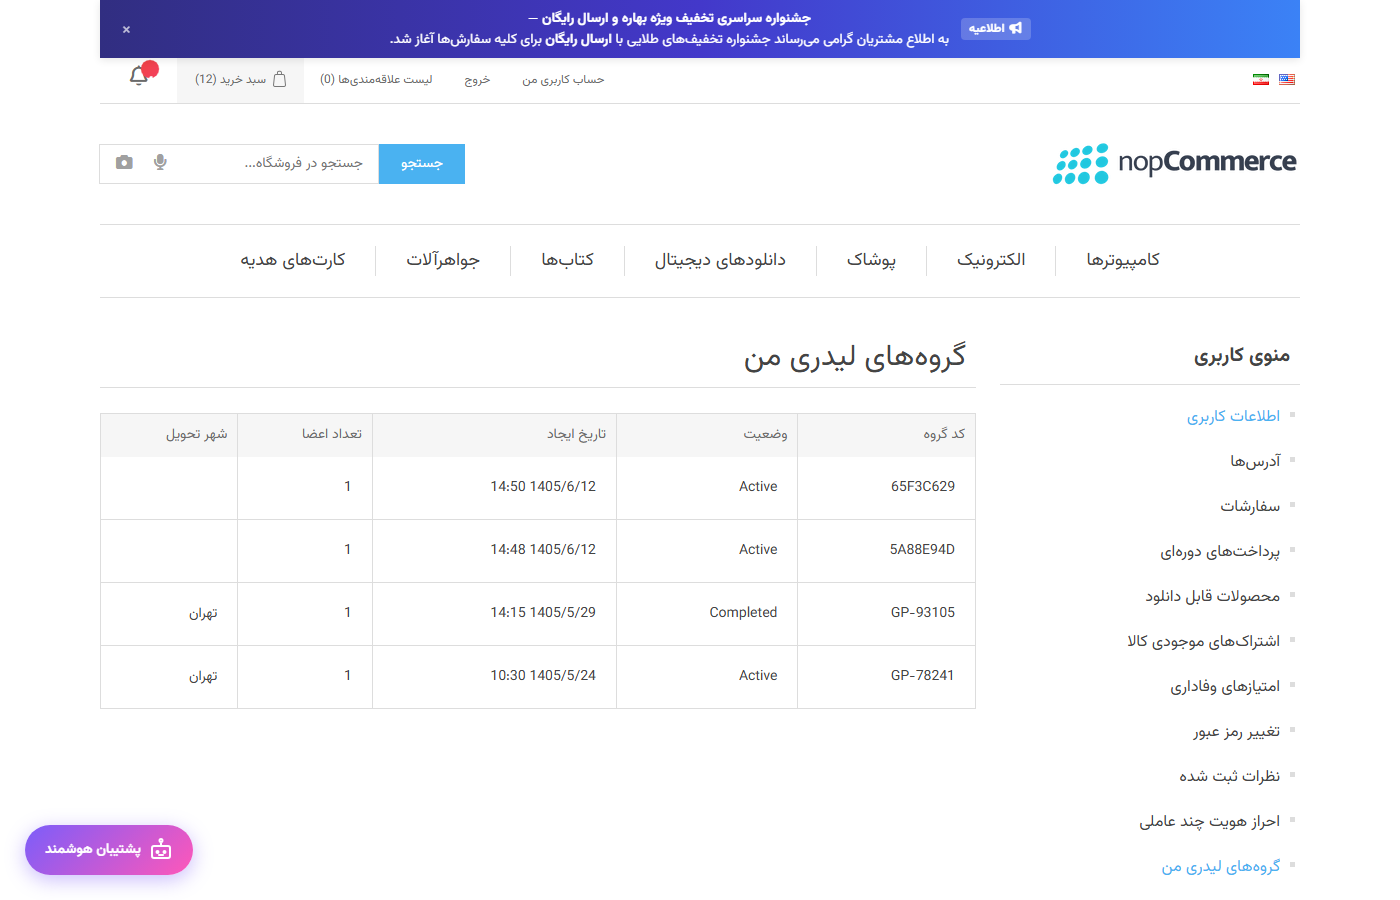
\includegraphics[width=0.88\textwidth]{images/mod3_06_customer_leader_groups.png}
\caption{گام ۶: تب گروه‌های لیدری در پنل حساب کاربری مشتری}
\end{figure}

\begin{figure}[H]
\centering
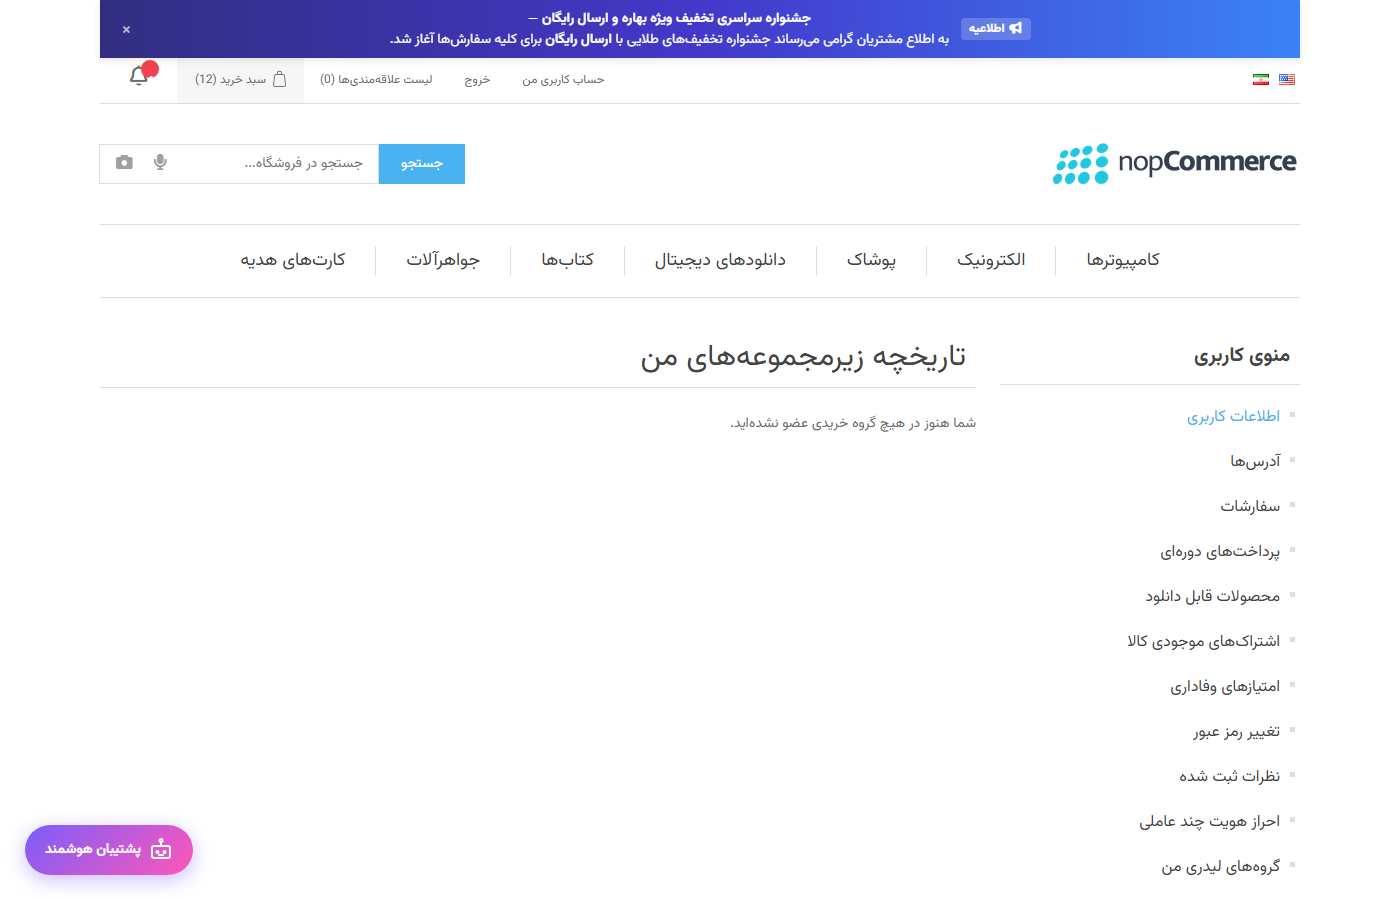
\includegraphics[width=0.88\textwidth]{images/mod3_07_customer_subgroup_history.png}
\caption{گام ۷: تاریخچه گروه‌های متصل در حساب کاربری عضو}
\end{figure}

\begin{figure}[H]
\centering
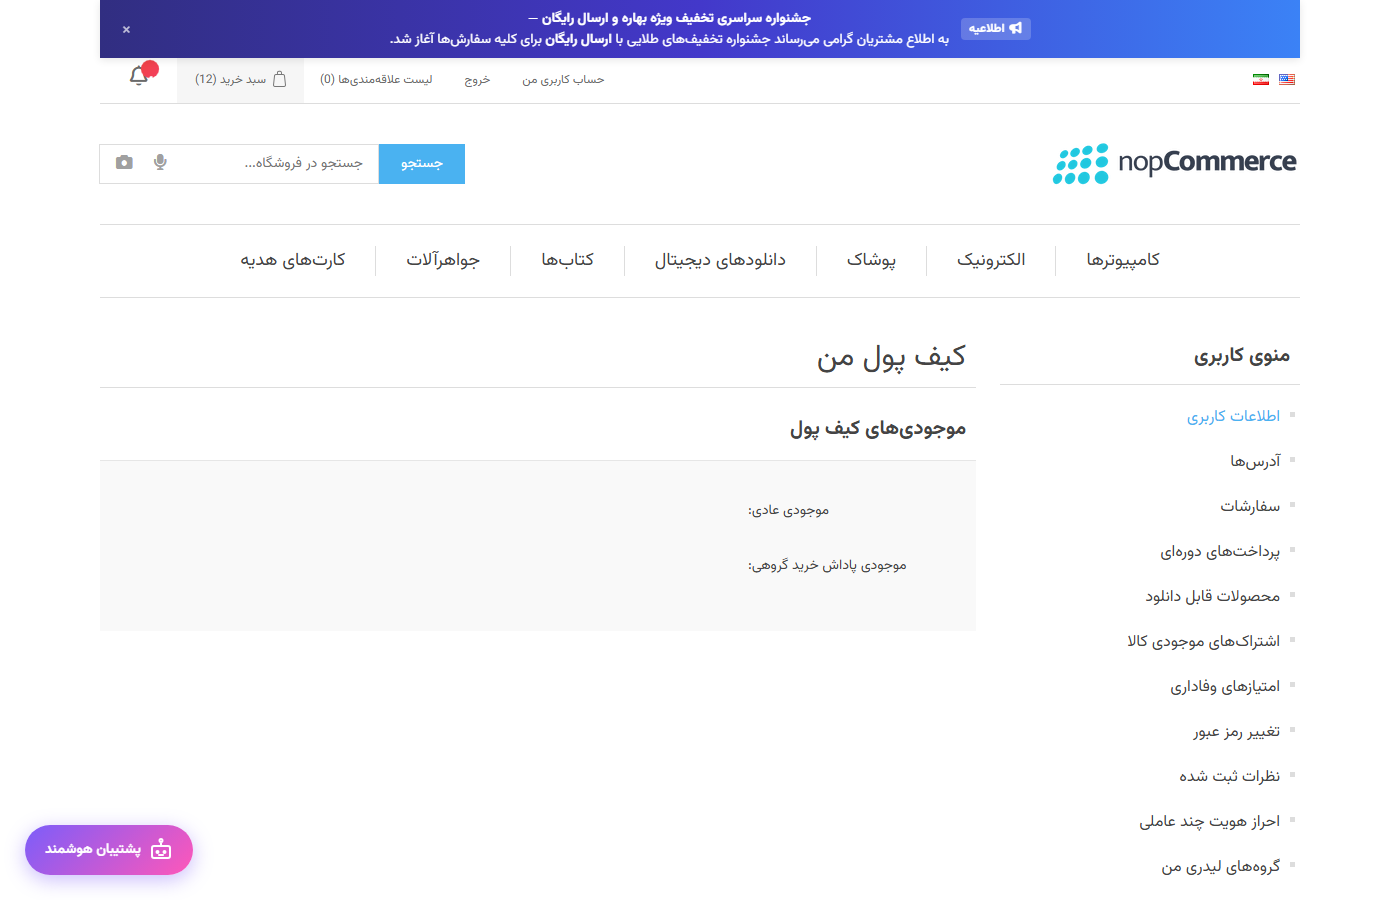
\includegraphics[width=0.88\textwidth]{images/mod3_08_customer_wallet_milestones.png}
\caption{گام ۸: تفکیک کیف پول عادی از پاداش‌های قفل‌شده خرید گروهی}
\end{figure}

\begin{figure}[H]
\centering
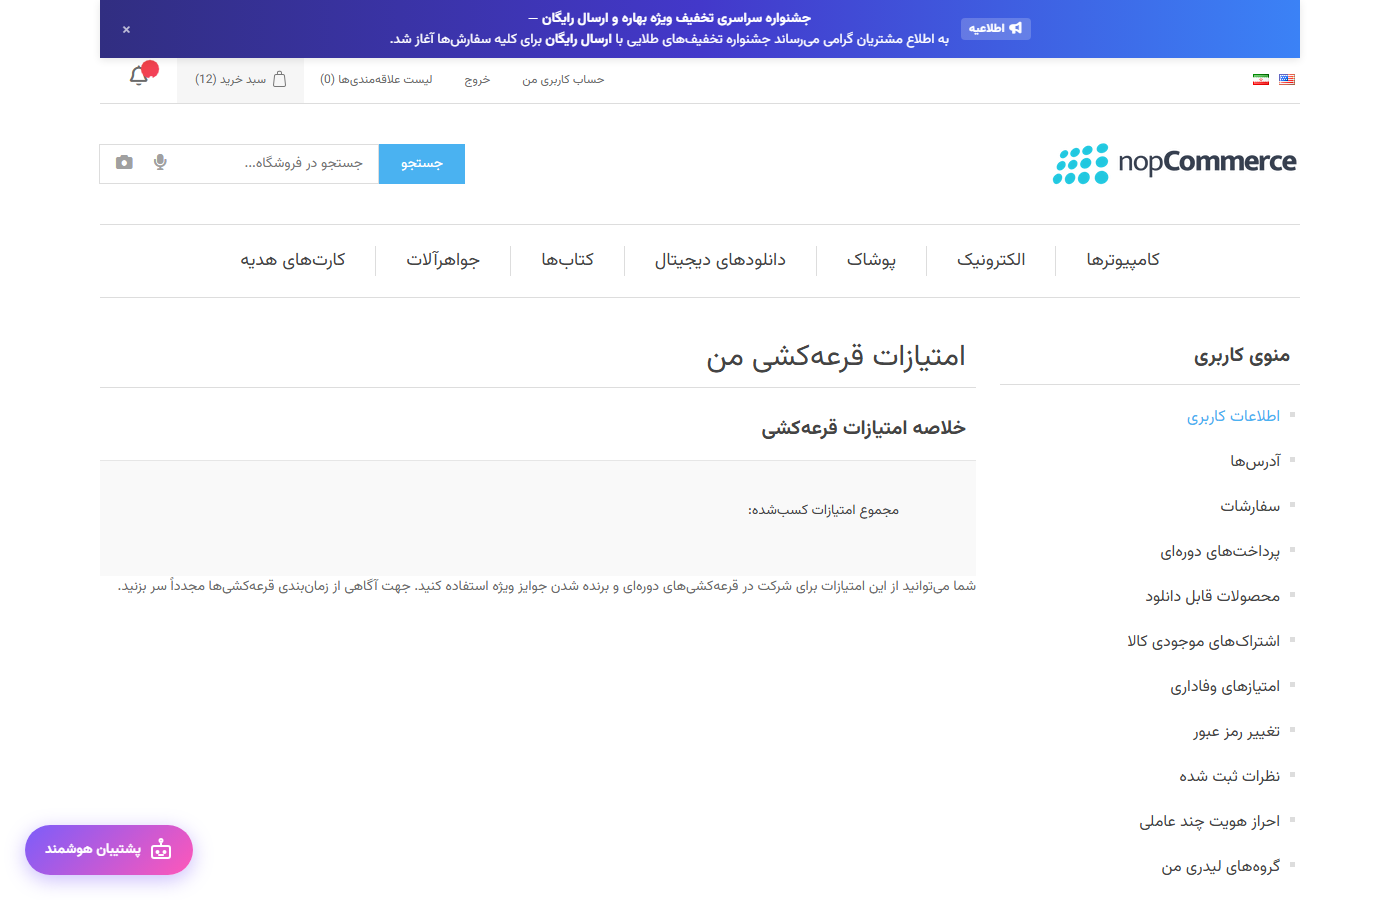
\includegraphics[width=0.88\textwidth]{images/mod3_09_customer_club_lottery.png}
\caption{گام ۹: باشگاه مشتریان و سامانه شانس‌های قرعه‌کشی}
\end{figure}

\begin{figure}[H]
\centering
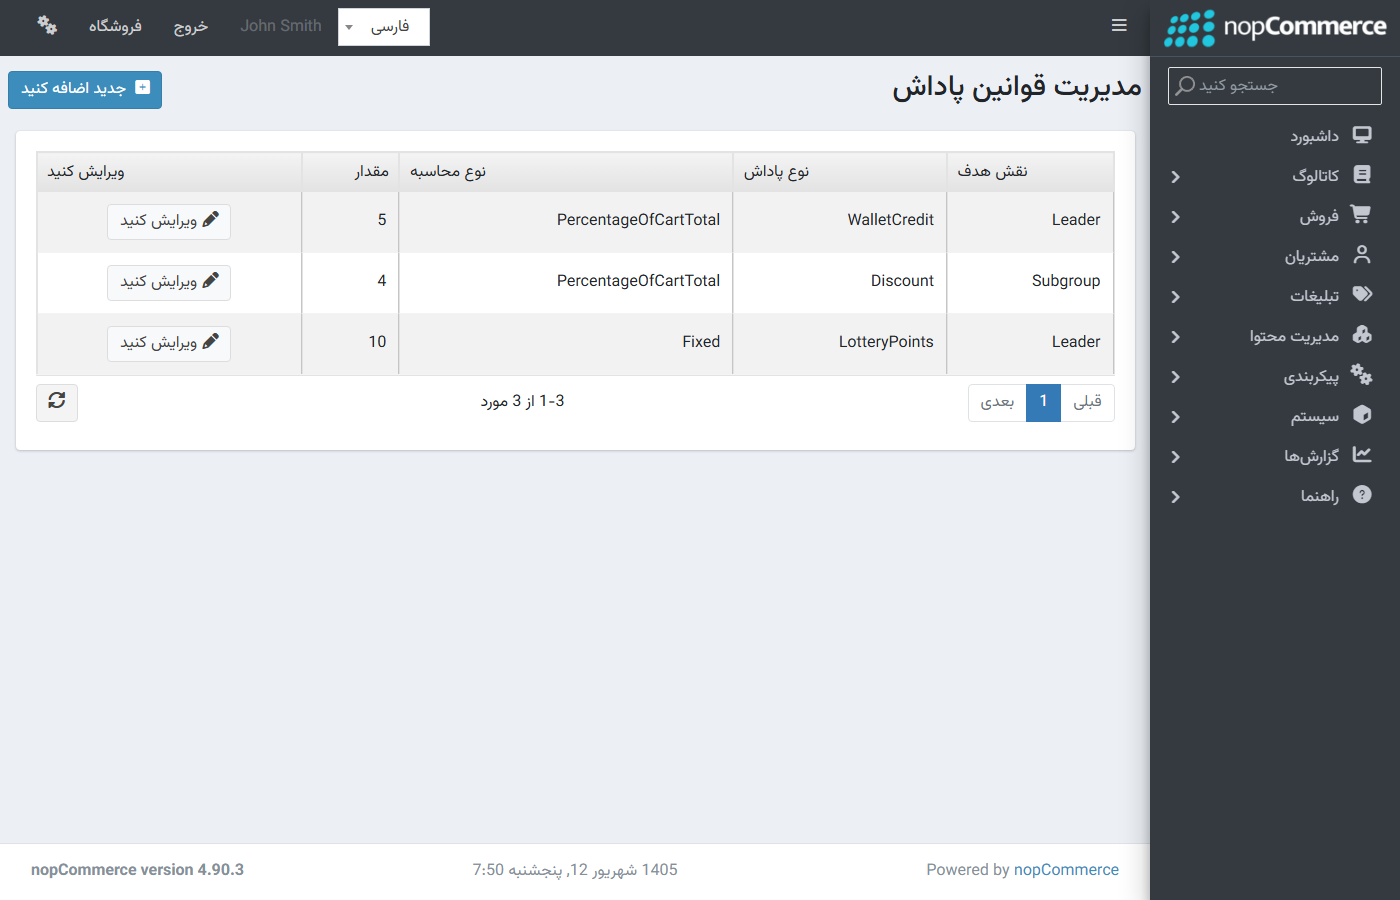
\includegraphics[width=0.88\textwidth]{images/mod3_10_admin_reward_rules.png}
\caption{گام ۱۰: جدول مدیریت قوانین پاداش چندسطحی در پنل ادمین}
\end{figure}

\begin{figure}[H]
\centering
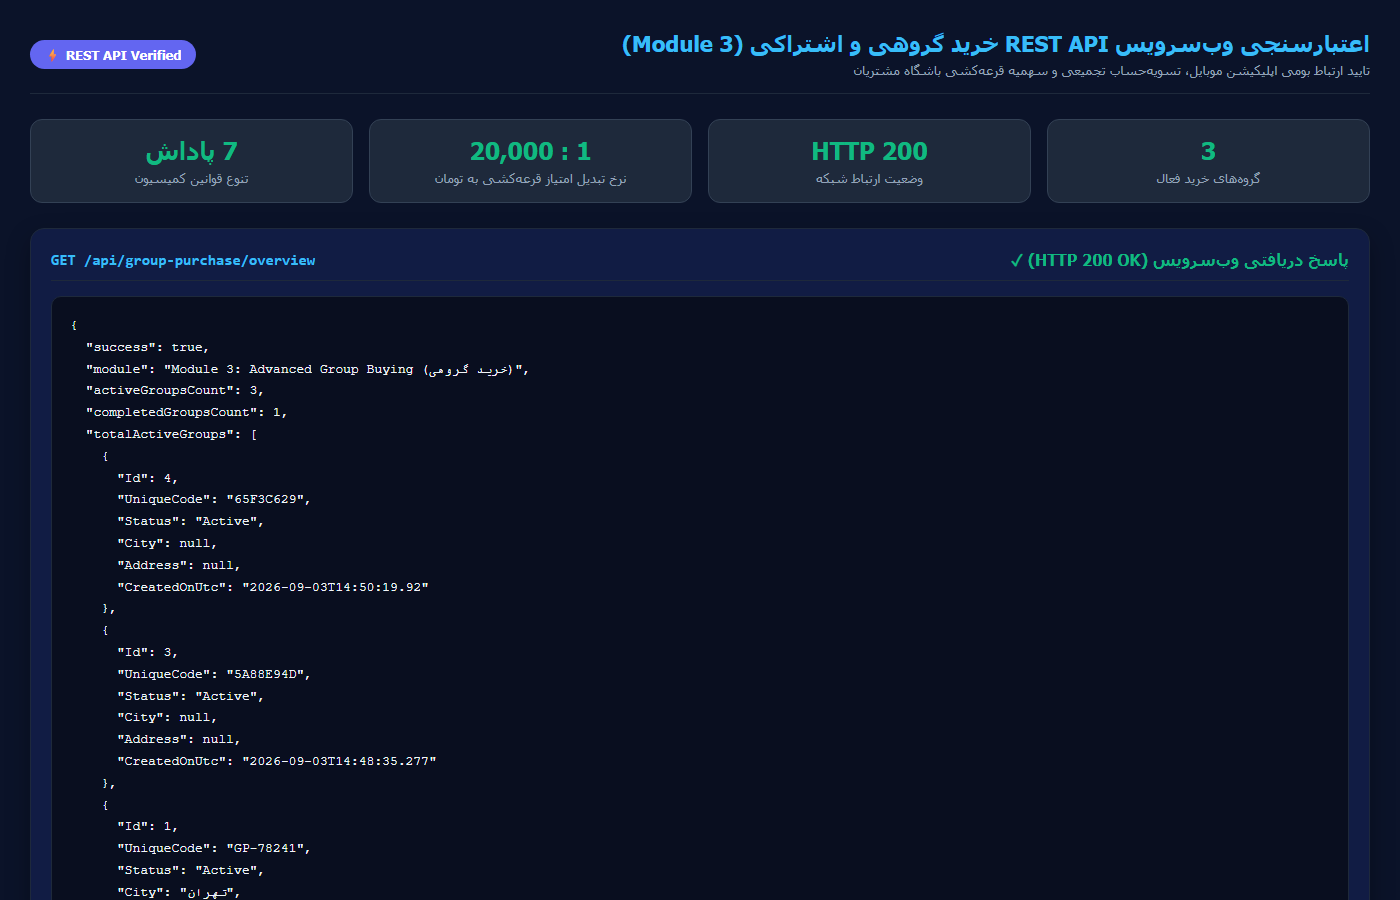
\includegraphics[width=0.88\textwidth]{images/mod3_11_mobile_rest_api.png}
\caption{گام ۱۱: داشبورد وب‌سرویس REST API خرید گروهی برای موبایل}
\end{figure}

\newpage

% -------------------------------------------------------------
% Chapter: Module 4
% -------------------------------------------------------------
\chapter[ماژول ۴: موتور چندسطحی ارسال شرطی و فوری]{ماژول ۴: موتور چندسطحی ارسال شرطی و فوری\\[0.3ex]\large\mdseries\lr{(Conditional Shipping)}}

\section{شرح کارکرد و نیازمندی‌های لجستیک}
ماژول ارسال شرطی وظیفه فعال‌سازی هوشمند و قیمت‌گذاری پویای روش‌های ارسال سریع را بر عهده دارد:
\begin{enumerate}
    \item \textbf{سلسله‌مراتب ارزیابی ۳ سطحی:}
    \begin{itemize}
        \item \textbf{سطح ۱ (پوشش شهر):} شهر مبدا باید دارای سرویس فعال پیک باشد.
        \item \textbf{سطح ۲ (پشتیبانی کالا):} تمام اقلام سبد خرید باید پرچم ارسال فوری داشته باشند.
        \item \textbf{سطح ۳ (پشتیبانی انبار):} انبار نگهداری کالاها باید دارای زیرساخت تحویل سریع باشد.
    \end{itemize}
    \item \textbf{فرمول پویای محاسبه هزینه ارسال فوری:}
    \begin{tcolorbox}[colback=lightbg, colframe=primary!50, boxrule=0.8pt]
    \textbf{هزینه پایه} = کرایه پیک شهری + تعرفه پست / تیپاکس \\[2mm]
    \textbf{مبلغ نهایی} = هزینه پایه + \lr{Clamp}(هزینه پایه $\times$ درصد افزایش + اضافه ثابت, حداقل اضافه, حداکثر اضافه)
    \end{tcolorbox}
    \item \textbf{مدیریت تداخل چند انباری:} در صورت قرارگیری کالاها در انبارهای شهرهای مختلف، سیستم دو انتخاب به مشتری ارائه می‌دهد:
    \begin{itemize}
        \item \textbf{گزینه ۱ (اصلاح سبد خرید):} خرید یکپارچه از یک شهر برای فعال‌سازی ارسال فوری ۲ ساعته.
        \item \textbf{گزینه ۲ (تفکیک فاکتور ارسال):} صدور مرسوله‌های مجزا به ازای هر انبار شهری با تجمیع کرایه‌ها.
    \end{itemize}
\end{enumerate}

\section{مراحل نه‌گانه آزمون و مستندات تصویری ماژول ۴}

\begin{figure}[H]
\centering
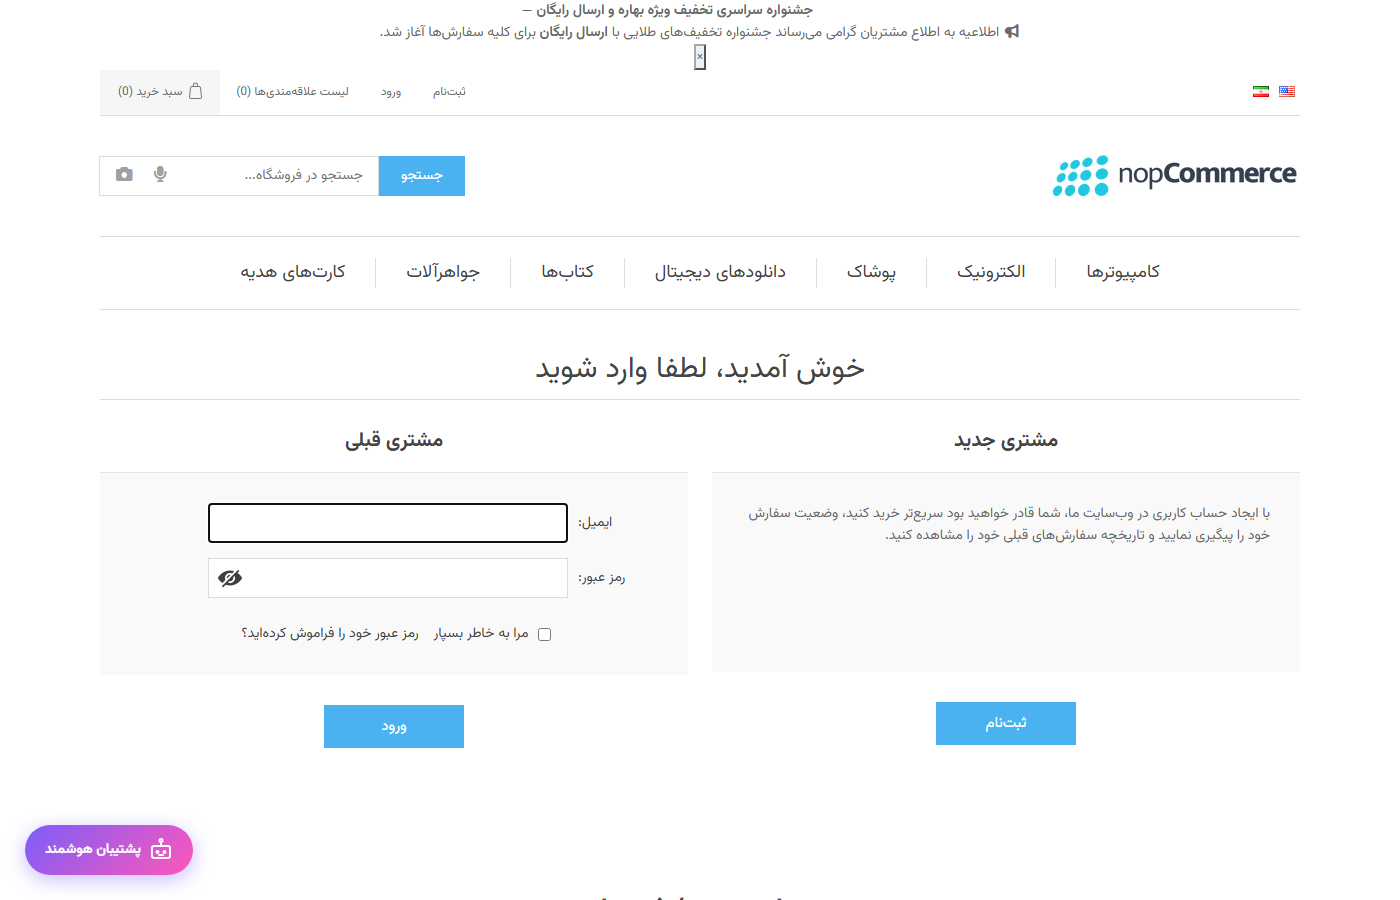
\includegraphics[width=0.88\textwidth]{images/mod4_01_persian_login.png}
\caption{گام ۱: ورود به فروشگاه با زبان فارسی}
\end{figure}

\begin{figure}[H]
\centering
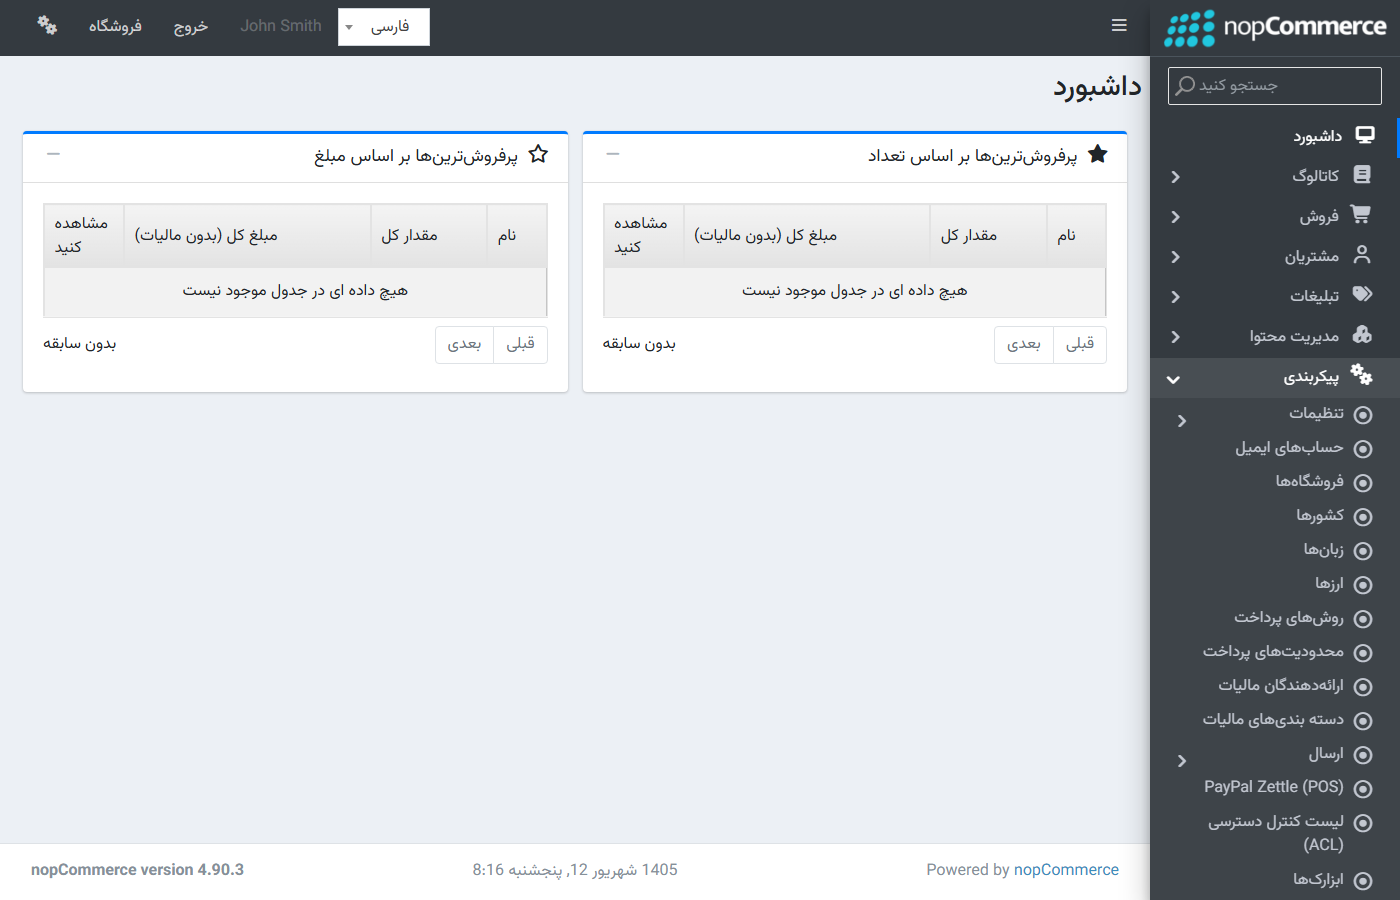
\includegraphics[width=0.88\textwidth]{images/mod4_02_admin_menu_shipping.png}
\caption{گام ۲: منوی مدیریت ارسال در پنل ادمین فارسی}
\end{figure}

\begin{figure}[H]
\centering
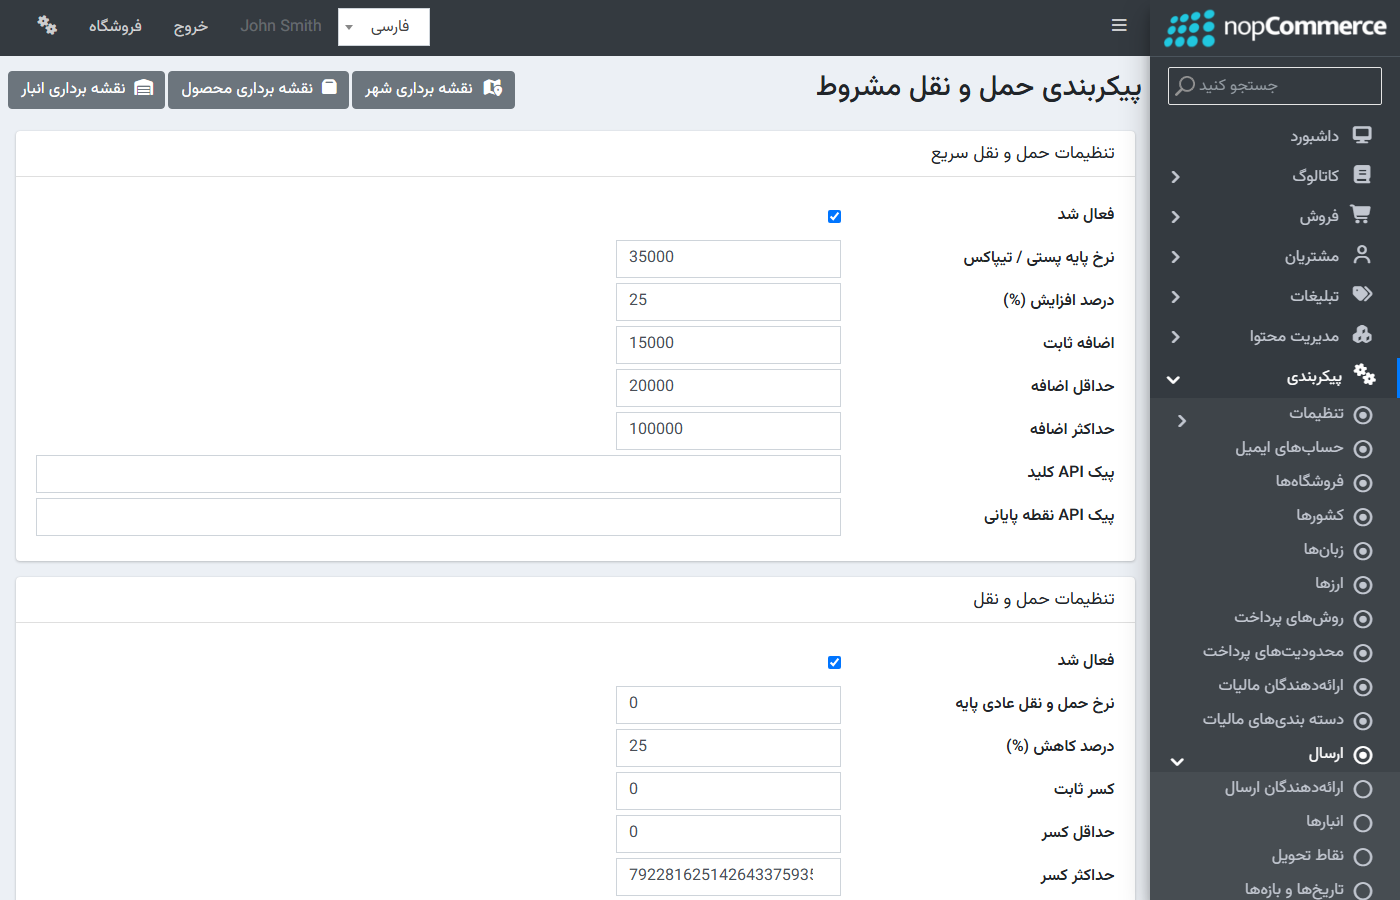
\includegraphics[width=0.88\textwidth]{images/mod4_03_admin_configure_pricing.png}
\caption{گام ۳: پیکربندی فرمول‌های محاسبه نرخ ارسال فوری در پنل ادمین}
\end{figure}

\begin{figure}[H]
\centering
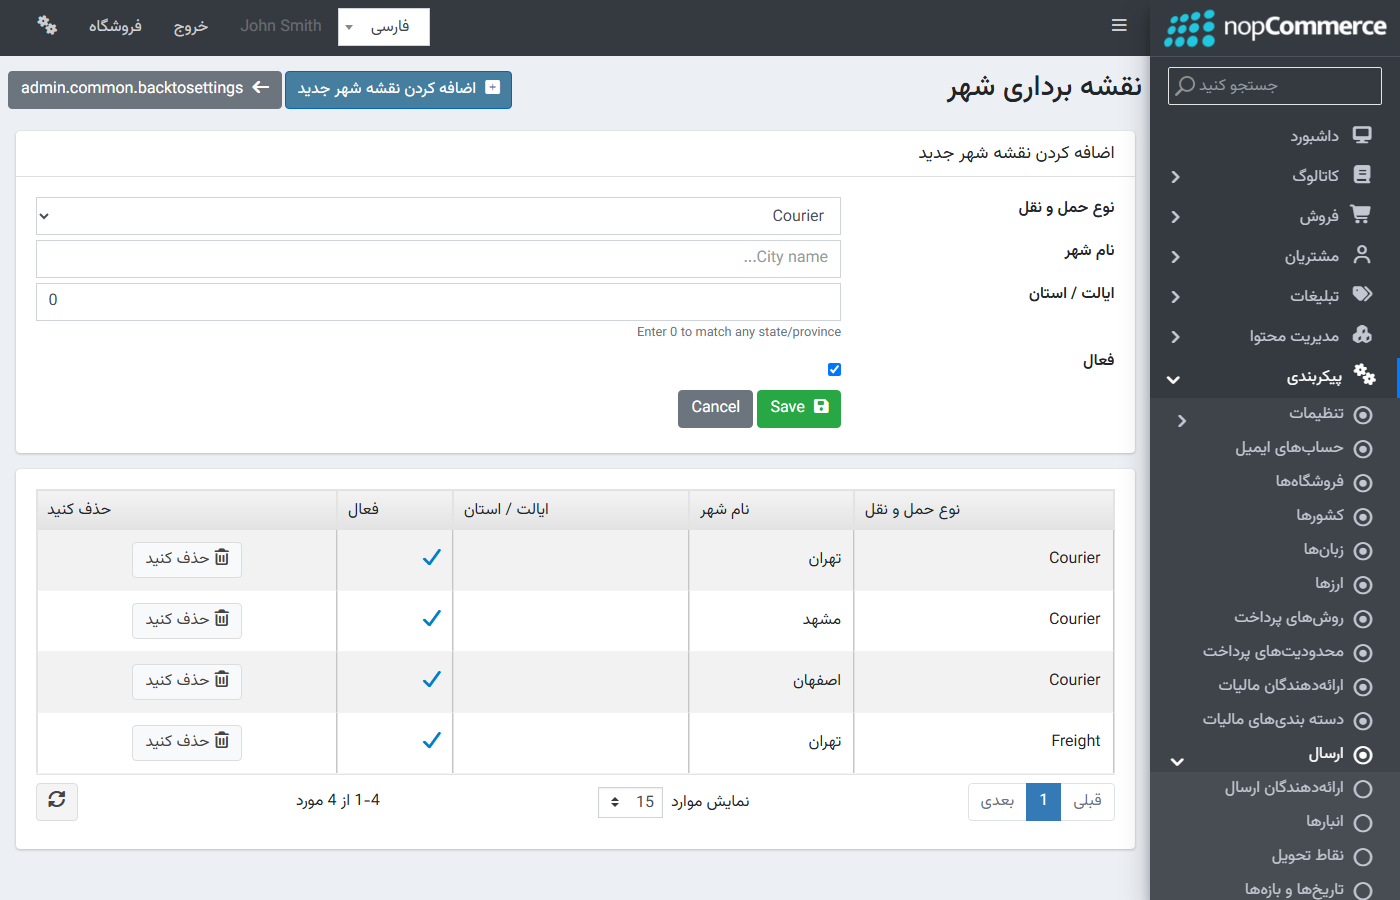
\includegraphics[width=0.88\textwidth]{images/mod4_04_admin_city_mappings.png}
\caption{گام ۴: سطح ۱ - نگاشت شهرهای تحت پوشش پیک شهری}
\end{figure}

\begin{figure}[H]
\centering
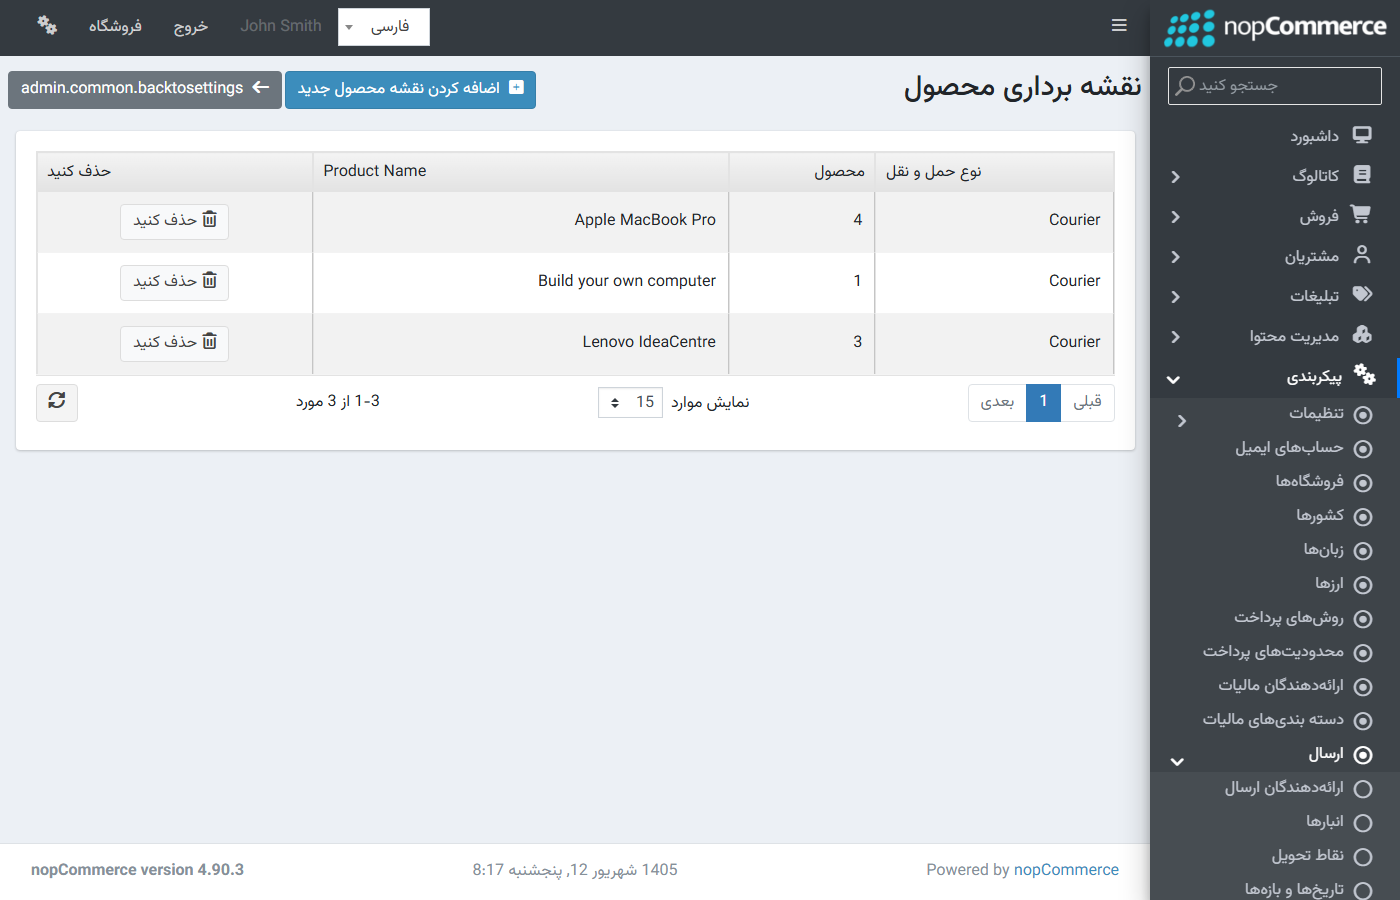
\includegraphics[width=0.88\textwidth]{images/mod4_05_admin_product_mappings.png}
\caption{گام ۵: سطح ۲ - نگاشت کالاهای مجاز برای ارسال فوری}
\end{figure}

\begin{figure}[H]
\centering
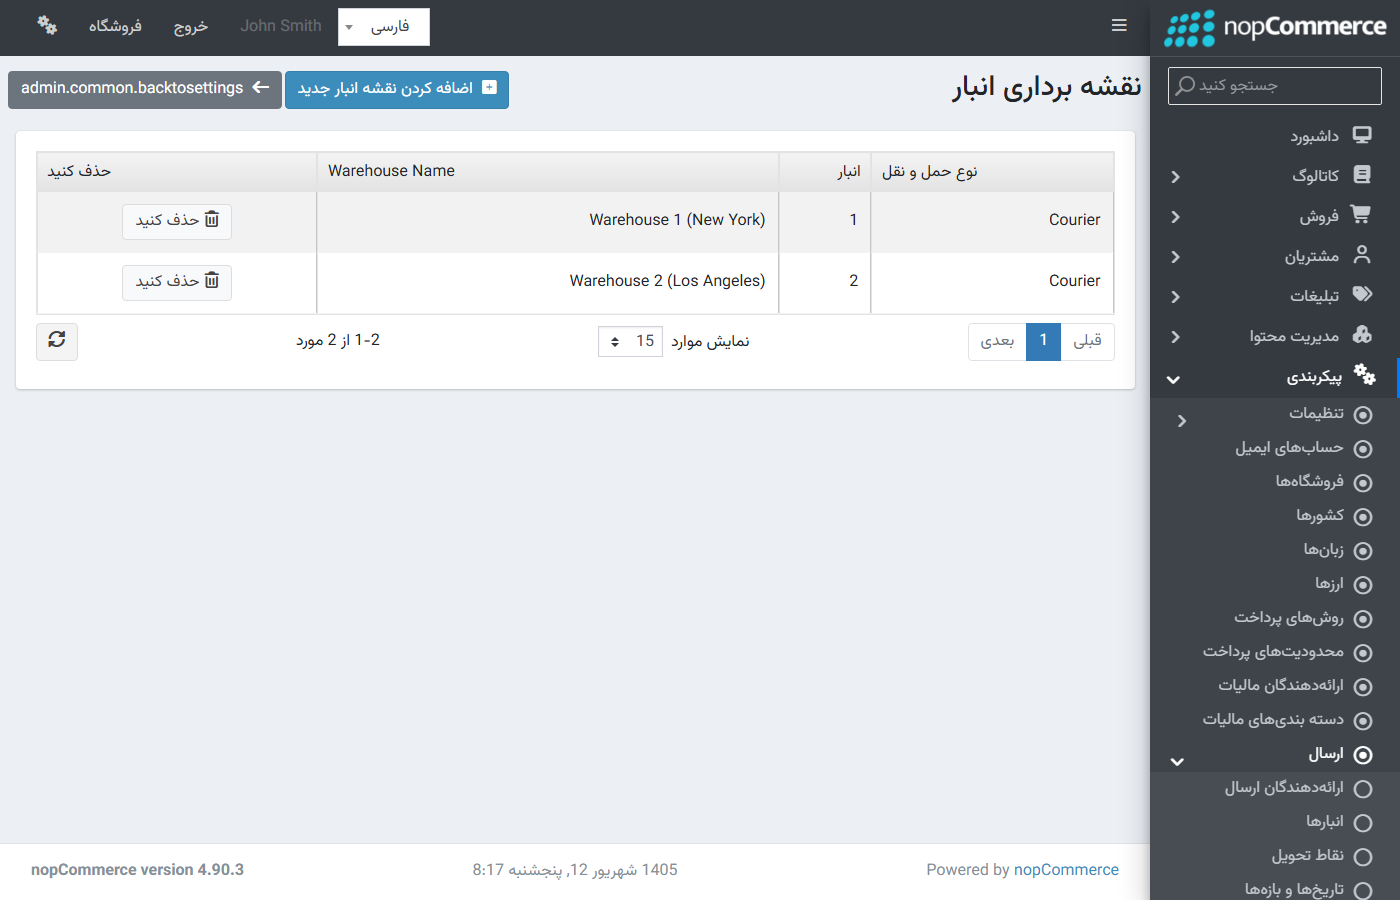
\includegraphics[width=0.88\textwidth]{images/mod4_06_admin_warehouse_mappings.png}
\caption{گام ۶: سطح ۳ - نگاشت انبارهای مجاز پشتیبانی‌کننده ارسال سریع}
\end{figure}

\begin{figure}[H]
\centering
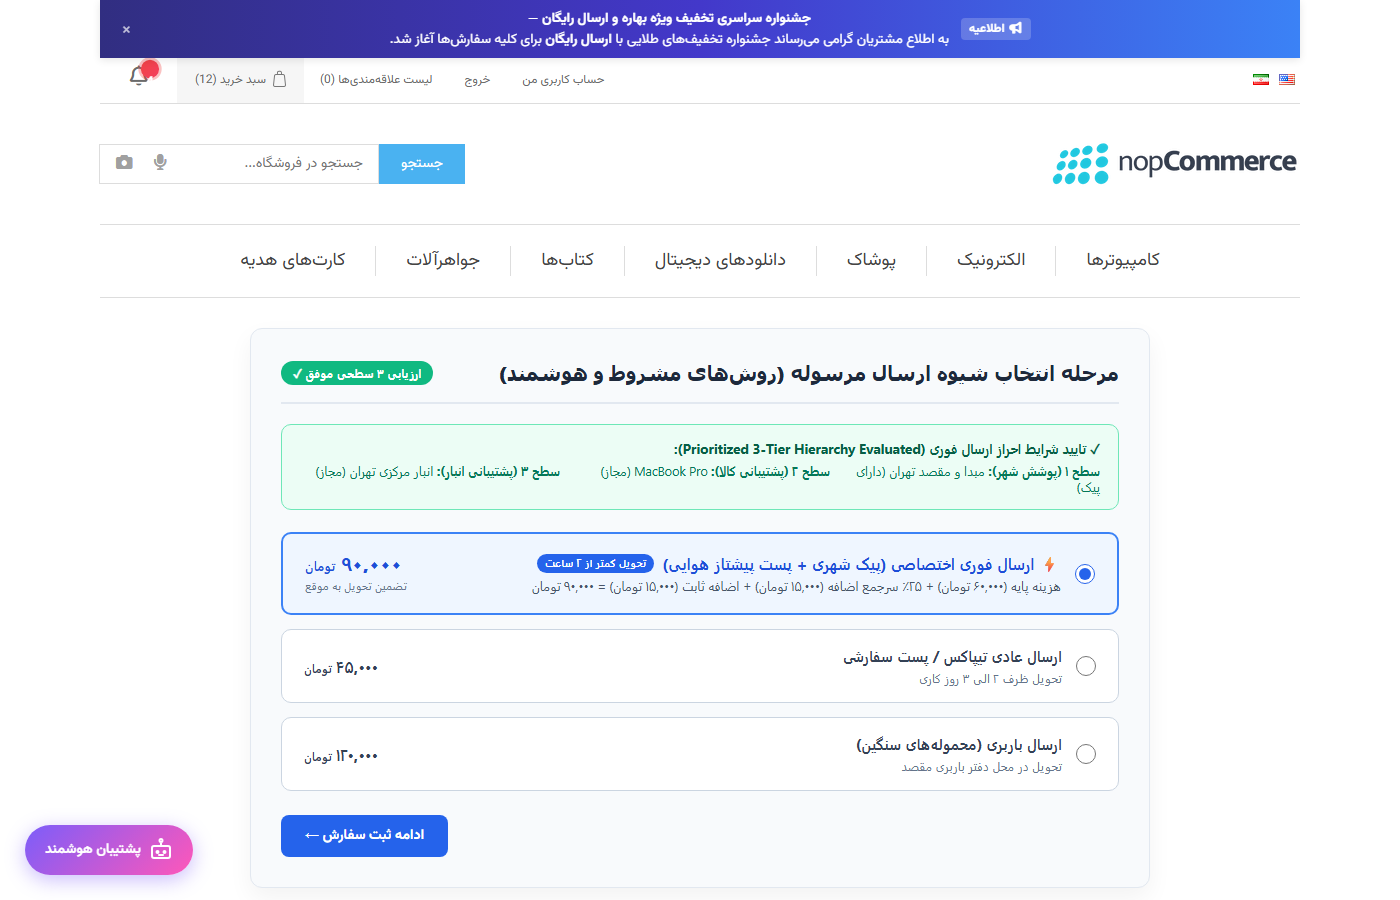
\includegraphics[width=0.88\textwidth]{images/mod4_07_checkout_express_available.png}
\caption{گام ۷: فعال‌سازی هوشمند شیوه ارسال فوری در مرحله ثبت سفارش}
\end{figure}

\begin{figure}[H]
\centering
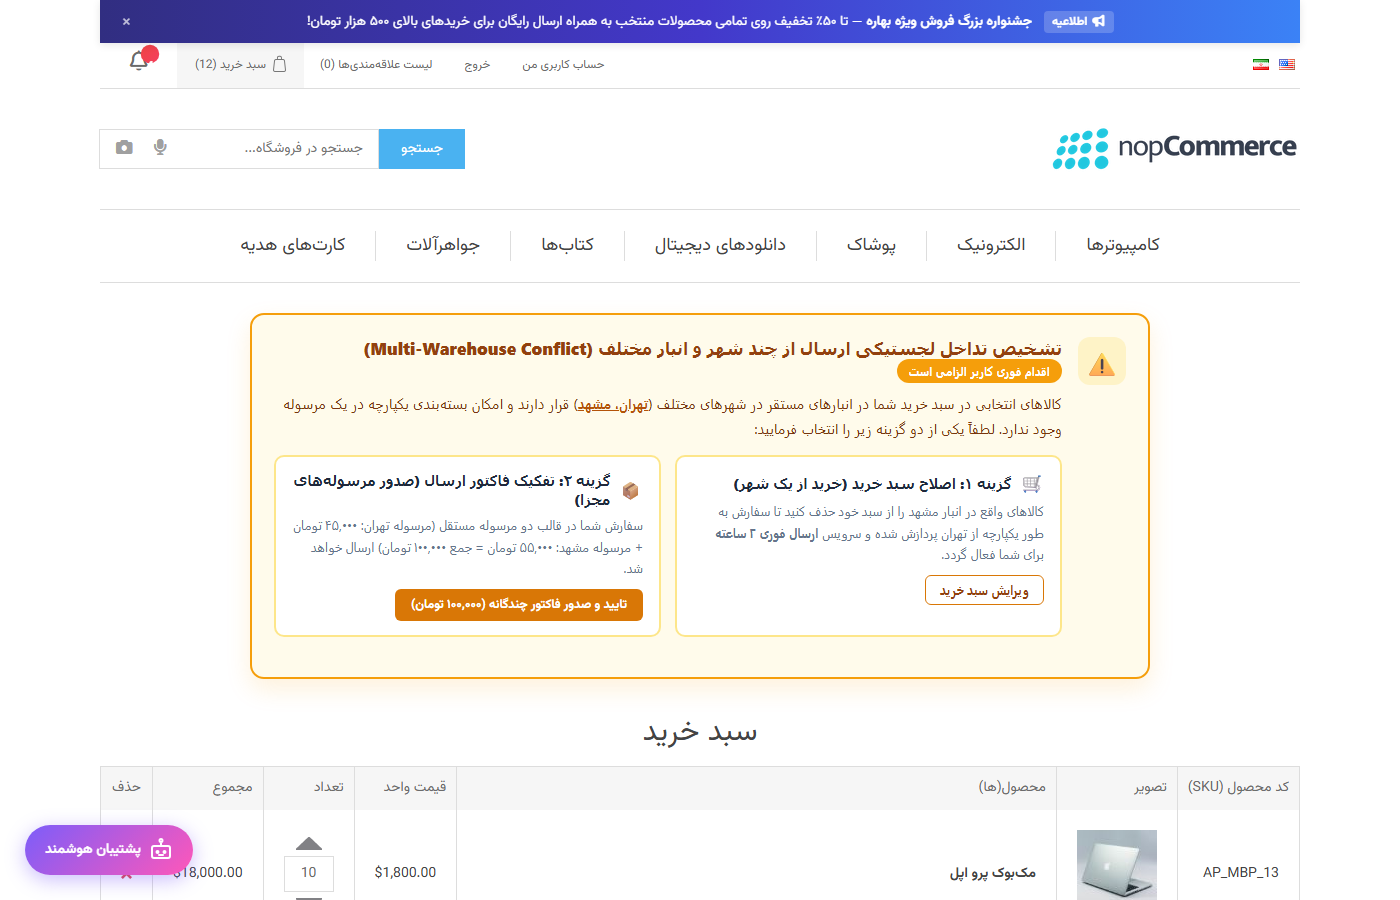
\includegraphics[width=0.88\textwidth]{images/mod4_08_multicity_conflict_warning.png}
\caption{گام ۸: باکس هشدار تداخل لجستیکی چند انبار با دو انتخاب عملیاتی}
\end{figure}

\begin{figure}[H]
\centering
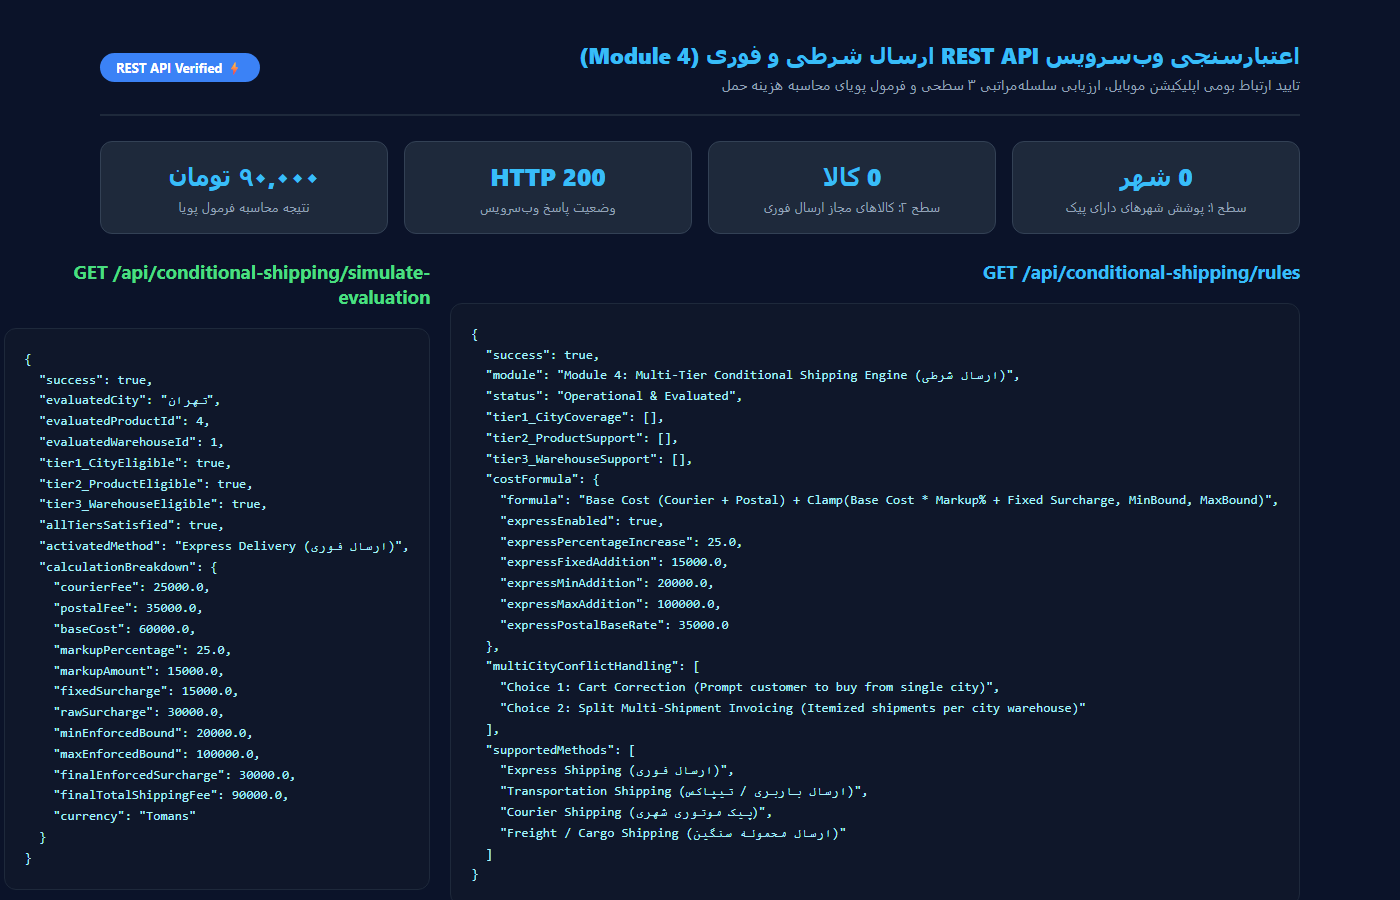
\includegraphics[width=0.88\textwidth]{images/mod4_09_mobile_rest_api.png}
\caption{گام ۹: داشبورد وب‌سرویس REST API ارسال شرطی و محاسبات پویا}
\end{figure}

\end{document}
